%\documentclass[a4paper, 12pt, twoside,parskip=half]{scrbook} 
\documentclass[a4paper,oneside, 12pt,parskip=half]{scrbook} 

% Increase margins to make todo items more readable during review
% process.

% === OLD VALUE ===
% \usepackage[left=2cm, right=2cm, bottom=2cm, top=2cm]{geometry}

% === SB Addition for review ===
\usepackage[left=2cm, right=7cm, bottom=2cm, top=2cm, marginparwidth=6cm]{geometry}
\usepackage{setspace}
\doublespacing
% \usepackage{showframe}
% ==============================


\usepackage[pdftex, breaklinks, colorlinks, citecolor=blue, urlcolor=blue]{hyperref}
\usepackage{graphicx}
\usepackage{float}
\graphicspath{{figures/}}
\usepackage{fancyhdr}
\pagestyle{fancy}
\fancyhf{}
\fancyhead[EL]{\thepage}
\fancyhead[ER]{\leftmark}
\fancyhead[OL]{\rightmark}
\fancyhead[OR]{\thepage}
\usepackage{etoolbox}
% % add bib to toc
\usepackage[nottoc,numbib]{tocbibind}
\usepackage[bibencoding=utf8, sorting=none]{biblatex} 
\addbibresource{references.bib}
\usepackage{amssymb}
\usepackage{mathtools}

\usepackage{todonotes}




%\renewcommand\chapterheadstartvskip{\addvspace{-0ex}}
%\renewcommand{\chapterheadstartvskip}{\vspace{0pt}}



%\RedeclareSectionCommands[
%beforeskip=-1sp,
%afterskip=1.2pt
%]{section,subsection,subsubsection}

%\RedeclareSectionCommand[
%runin=false,
%beforeskip=-1sp,
%afterskip=-\parskip
%]{section}

%\RedeclareSectionCommand[
%runin=false,
%beforeskip=-1sp,
%afterskip=-\parskip
%]{subsection}

% \RedeclareSectionCommand[style=section,indent=0pt]{chapter}
%\addtokomafont{chapter}{\fontsize{18}{18}\selectfont}
\addtokomafont{section}{\fontsize{11}{12}\selectfont}
\addtokomafont{subsection}{\fontsize{10}{11}\selectfont}

\usepackage{caption}
\captionsetup[figure]{font=footnotesize}


% % ================= FRONT MATTER ================================
\begin{document}
\begin{titlepage}

\begin{center}
	
\includegraphics[width=0.4\textwidth]{figures/usyd_logo}
\end{center}
	\vspace{2cm}
\begin{center}
	\LARGE\textbf{Clinical application of deep learning: \\ Automatic contouring via U-net architecture}
	\vfill

	% Set font back to normal size
	\normalsize
  \large{\textbf{Matthew Cooper}}
  \vfill
	
	\normalsize
	Supervised by:

	Simon Biggs, Riverina Cancer Care Centre
  
	Dr. Yu Sun, University of Sydney
  
	Matthew Sobolewski, Riverina Cancer Care Centre 
	
	\vspace{1cm}
	
	\textit{In partial fulfilment of the requirements for the degree Master of Medical Physics}
	
	\vspace{1cm}
	
	Institute of Medical Physics
	
	School of Physics
	
	The University of Sydney
	
\vspace{1cm}
June 2020
	\vfill
  \end{center}
\end{titlepage}

\frontmatter
% % Table of contents: 4 (Only on page counts towards limit)
\tableofcontents
% % Abstract: page 2 - 200w or less
\chapter{Abstract}
\label{ch:abstract}

\textbf{Purpose:} Accurate contouring is a critical aspect of safe and effective treatment delivery in radiotherapy (RT). Current limitation in clinical practice include:\todo{is this punctuation correct here?} Large inter and intra-observer variances, as well time delays in both contour generation and correction - that act as barriers to the implementation of adaptive RT\todo{This feels like you're introducing a list, but there is only one item in it...}. This study designs and evaluates a 2D U-net\todo{U-Net?} architecture with two primary aims: 1) Develop a pelvic imaging quality assurance tool for use in RT, comparing model predictions with expert contours. 2) Automate vacuum bag segmentation for canine RT.

\textbf{Method:}
 We present two independently trained models in this study, and assess the performance of common semantic segmentation loss functions in each case. We expand on the original architecture developed by Ronneberger et al. by integrating recent network modifications that have shown improved performance in the literature. In addition to reporting dice similarity (DSC), we utilise organ-specific tolerances representative of expert IOV for the bladder and rectum as parameters in Nikolov et al's surface dice similarity coefficient (sDSC).

\textbf{Results:}
3 \todo{Three} contours were produced from pelvic imaging CT scans: Patient contours were measured with mean DSC 0.99(0.01)\todo{No sDSC?}, bladder contours with mean DSC 0.86(0.22) and mean\todo{No need to repeat 'mean' here} sDSC 0.87(0.18), and rectum contours with mean\todo{nor here} DSC 0.67(0.12) and mean sDSC 0.92(0.14). Additionally, vacuum bag contours from canine imaging CT scans were measured with mean DSC 0.95(0.01)\todo{sDSC?}. Weighted DSC was the only loss function that optimised for all organs considered in pelvic imaging - due to a significant class imbalance \todo{class imbalance 'by relative contour pixel volume'?}.

\textbf{Conclusion:}
Patient contours were excellent\todo{"Excellent" -- not scientific language. Instead something like "Patient contours did not deviate outside tolerances and are viable for use within the QA tool in their current form"}. We\todo{Would "it is suspected" be better here?} suspect a broader dataset may improve bladder and rectum segmentations (19 patient scans were used). The vacuum bag model should proceed to acceptance testing for clinical implementation.

\chapter{Acknowledgements}
\label{ch:acknowledgements}

The author wishes to acknowledge the following:

\textbf{Simon Biggs}

For his mentorship and support over the course of the project. Simon played a pivotal role
in shaping the author's philosophy of code development. In addition, he facilitated the
author's first professional connections within the medical physics community.

\textbf{Dr. Yu Sun}

For his encouragement and guidance throughout the Master of Medical Physics degree. Yu Sun has also been key in expanding the author's professional network - increasing the exposure of this project.

\textbf{Matthew Sobolewski}

Matthew provided valuable feedback and guidance on both the presentation and the research report. The author wishes to thank Matthew for supporting the first student research project at Riverina Cancer Care Centre.

\textbf{The teams at Riverina Cancer Care Centre \& the Small Animal Specialist Hospital}

In particular: Jacob McAloney, Nick Menzies, and
Simon Biggs, for providing accommodation in their own homes over the course of
the project. This allowed the author to gain formative clinical experience. Additionally, this project would not have been possible without the data provided by Riverina Cancer Care Centre (RCCC) and the Small Animal Specialist Hospital (SASH). The medical physics team at RCCC also provided valuable feedback on the presentation.


\textbf{Dr. Annette Haworth \& Dr. Sianne Oktaria}

For going above and beyond to ensure March--June 2020 research students were able to complete their projects on time and remotely during the COVID-19 pandemic.

\textbf{Dr. Robert Finnegan}

For providing detailed feedback on the presentation.

\textbf{The team at DeepMind}

For making public their surface-distance-based performance metrics.

\url{https://github.com/deepmind/surface-distance}

\chapter{Statement of contribution}
\label{ch:contribution}

This project was suggested by Simon Biggs and was presented with the freedom to explore any solution that the author believed would have clinical application. All research was conducted by the author; although, Simon suggested Nikolov et al. as an initial blueprint. All code used in this project (except for common machine learning and computational packages) was written by the author and has been released under an open-source license. Additionally, the author built a custom PC with the GPU used for computation in this project - NVIDIA RTX 2070 Super. Simon Biggs organised access to clinical data on site at Riverina Cancer Care Centre (RCCC), and provided a software solution for anonymising patient scans. Furthermore, Simon Biggs organised canine imaging data from the Small Animal Specialist Hospital (SASH) after suggesting that this would be a good place to start getting familiar with coding libraries. In addition to the above, Simon Biggs and Yu Sun provided weekly to bi-weekly feedback on the project direction over the course of the semester.


\textbf{Code repository:} \href{https://github.com/pymedphys/pymedphys}{github.com/pymedphys}


\vspace{1cm}
\vspace{1cm}

I certify that this report contains work carried out by myself except where otherwise
stated.
\\
\\
- Matthew Cooper     10/06/2020
\\
\\

% % List of tables and figures: 4 (Does not count towards limit)
\listoffigures
\listoftables

% % ================= MAIN MATTER =========================
\mainmatter
% Remove page numbering for new chapter pages
\fancypagestyle{plain}{%
  \renewcommand{\headrulewidth}{0pt}%
  \fancyhf{}%
}

% Introduction: 1-2 pages 
% Present background, motivation and rationale of project
\chapter{Introduction} \label{ch:introduction}

\section{Background}
Approximately 18 million patients are diagnosed with cancer each year \cite{Bray2019}, with reports indicating that up to 50\% of all cases could benefit from radiotherapy (RT) as curative or palliative management of disease (optimal radiotherapy utilisation rate) \cite{Barton2014}. 
Contouring is a critical aspect of RT treatment planning\todo{Is it worth spending one sentence at the beginning here describing what treatment planning itself actually is?}; it describes the process of defining and classifying anatomical regions-of-interest (ROIs) within a patient from medical imaging data \cite{CITATION}.
Contoured regions include: target volumes for treatment, associated error margins; as well as normal tissue regions} (organs at risk - OARs) - for which exposure needs to be minimised to avoid adverse side-effects of treatment \cite{CITATION}. Once ROIs are defined, beam output can be translated to patient anatomy\todo{`beam output can be translated to patient anatomy' reads awkwardly. Maybe, if you define what treatment planning is above, then you can just say here something like, `once the ROIs have been appropriately segmented they can be used within the dose prescription and optimisation stages of treatment planning'}, allowing for dose distributions to be determined for each region (as seen in Figure \ref{fig:contour}). Therefore, contours are part of the primary geometry used to optimise treatment outcomes; achieved by maximising tumour control probability and minimising normal tissue complication probability - i.e. maximising the therapeutic ratio of treatment\todo{The fact that increasing the theraptic ratio is the aim of all this means it likely should be towards the beginng, likely rolled into your treatment planning definition} by optimally distributing dose \cite{CITATION}. As such, accurate contouring is fundamental to the efficacy of RT \cite{CITATION}.

\begin{figure}[!htb]
	\begin{center}
		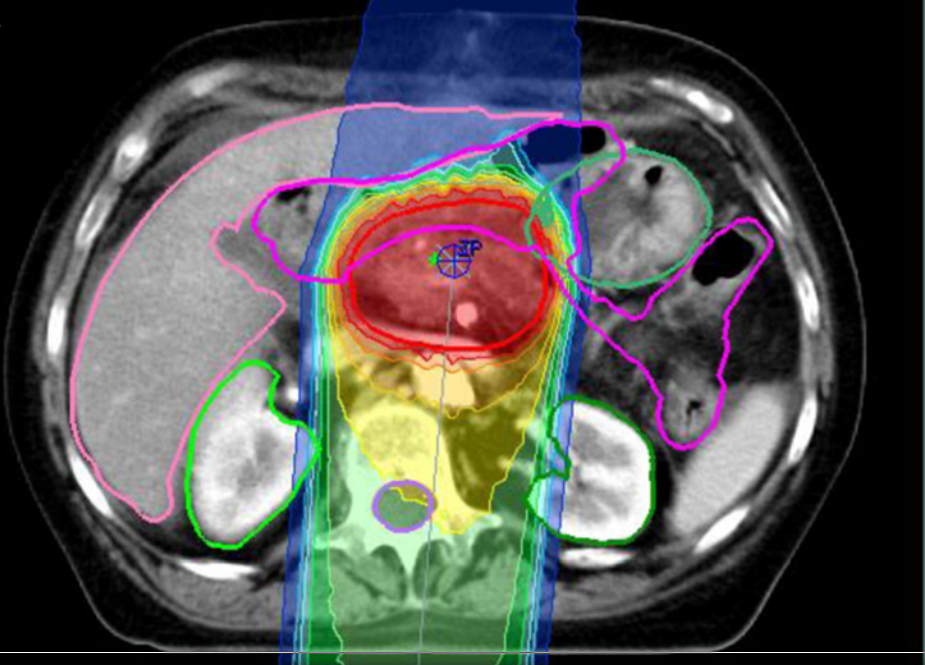
\includegraphics[width=0.5\textwidth]{contour}
		\caption{Single posterior field setup for carbon ion radiotherapy treatment of pancreatic cancer. Multiple contours are outlined on diagnostic CT imaging for treatment planning. Colour map shows the dose distribution over patient anatomy. Figure redrawn from Dreher et al. \cite{Dreher2017}.}
		\label{fig:contour}
	\end{center}
\end{figure}

However, there are current limitations in clinical practice. Large intra- and inter-practitioner (observer) variability (IOV) exists in the definition of ROIs on medical imaging. IOV is a long-standing challenge in RT, and is frequently reported as the largest source of error in accurate treatment delivery \cite{Vinod_2016, tg100}.
Additionally, manual contouring is both time consuming and requires skilled experts \cite{Nikolov_2018}. For instance, research has estimated that a radiation oncologist (RO) needs between 90 -- 120 minutes to delineate pelvic OARs in a cervical cancer patient \cite{Liu_2020}. The process is often computer aided and automatic OAR segmentation tools (i.e. deformable image registration or Atlas-based methods) have both reduced contouring times and improved consistency between expert observers \cite{Vinod_2016}. However, atlas-based methods still require significant manual editing \cite{Nikolov_2018}, and experience difficulty with small organ volumes, regions with poor contrast for differentiation, or high variability in size or location - such as pelvic OARs in prostate and cervical cancer \cite{Schreier_2020, Liu_2020}. Critically, current automatic solutions still present a barrier to the adoption of future technologies that would require fast contouring \cite{Nikolov_2018}. For instance, adaptive radiotherapy has shown the potential to deliver a new standard of care for RT patients by updating treatment plans to daily changes in patient anatomy \cite{Nikolov_2018}. 

In contrast, deep-learning (DL) algorithms have shown significant performance improvements over atlas-methods both in terms of accuracy and time for contour generation \cite{CITATION}. However, the implementation of DL models in clinical environments remains challenging; particularly due to limitations in quantitatively assessing model performance in comparison to expert performance and IOV \cite{Nikolov_2018}. Typical metrics used to quantify the similarity between model and expert contours are volumetric in nature, hence volume overlap tends to be the focus of evaluation \cite{Nikolov_2018}. Recent studies have introduced surface-based performance metrics that aim to provide direct information on the fraction of surface points that require correction to be within IOV tolerances (specific to each OAR) \cite{Nikolov_2018, Vaassen_2020}, and may provide a stronger correlation with time required for contour correction \cite{Vaassen_2020}.

\section{Aim}

U-Net is a type of deep-learning architecture that leverages multi-resolution analysis to perform state-of-the-art segmentation in medical imaging research \cite{Kazemifar_2018, Zhu_2018}\todo{This feels like we're still reading background\ldots}. We present two independent U-Net models in this study, and expand on the original architecture developed by Ronneberger et al. in \cite{Ronneberger_2015}, by integrating recent network\todo{This whole sentence feels like method. I don't believe one should so closely tie ``how it was implemented'' with ``what one sets out to achieve''.}  modifications that have shown improved performance in the literature: 

\textbf{Model 1 - Pelvic imaging QA tool}

Model 1 was designed to fulfil the need for contouring to become part of regular quality assurance due to large IOVs\todo{Actually, it wasn't primarily due to large IOVs, and to be honest here, if it was large IOVs your model shouldn't be designed pick up those issues, because it should let things pass if they are within IOVs. Instead, it is to catch gross contouring errors. An example might be a `left lens' contoured as a `right lens' or whole slices missing from a patient contour.} reported across the literature \cite{Vinod_2016}. In addition, model 1 aims to evaluate the ability of U-Net to achieve expert level performance - as defined by Nikolov et al.'s surface-based performance metric (surface dice similarity coefficient - sDSC) \cite{Nikolov_2018}. We focused on pelvic CT imaging scans, automatically contouring the patient, bladder and rectum volumes\todo{Add a note here about why these were chosen. They were considered to be the most easy organs to auto-contour in this way, chosen with the intent to act as a template for future work extending to other organs.}. The model then compares predicted contours with those created by an expert clinician; and provides feedback on the volumetric overlap (dice similarity coefficient - DSC), as well as the percentage of surface points that deviate by a distance larger than the IOV associated with each structure (sDSC). Recent studies have highlighted that surface overlap metrics - such as the sDSC - may have improved correlation with respect to manual correction times\todo{I believe you've already mentioned this in your lit-review, and if you haven't this should probably be removed from here and put there. -- potentially, remove all references to sDSC, U-Net, etc, and focus just on what the aim was, an aim that could have been fulfilled for example if you had of chosen an atlas method, no matter your method, the project aim didn't change.} required for an automatic segmentation, when compared with standard volumetric overlap metrics \cite{Vaassen_2020}. We present both metrics for comparison, with models trained over a variety of loss functions common to medical image segmentation.

\textbf{Model 2 - Automatic segmentation of vacuum bag structures in canine imaging}

Model 2 was designed to automatically contour vacuum bag structure in canine imaging. Vacuum bag structures are reported to take approximately 30 minutes per patient to contour \cite{CITATION}; hence, this model aims to automate a time-consuming aspect of RT treatment that is typically processed manually in veterinary medicine\todo{Maybe instead: `that is processed manually at the vetinary clinic in question.' It is not standard that vacbags are always contoured. Some clinics may ignore it entirely. Others draw large blobs around the whole thing.}.\todo{This is a much clearer aim}



% Literature review: Max 8 pages. T/f 6-8.
% A comprehensive review of relevant literature
\chapter{Literature} \label{ch:literature}

\section{Introduction}
Hardware developments in the last two decades (2000-2020) have enabled deep-learning algorithms to achieve state-of-the-art image segmentation in the field of computer vision, outperforming humans on many classification tasks \cite{ioffe2015, He2015, Wu2015}. The following review aims to cover recent developments in medical image segmentation by focusing on network architecture, training methods, and challenges in the context of radiotherapy (RT). We begin by examining variability in the definition of organs contoured by medical professionals, and outline a novel technique used by Nikolov et al. that takes this variability into account when assessing model performance \cite{Nikolov_2018}. Further, we explain U-net architecture in detail before expanding on the original work by examining modifications in recent implementations. We conclude the review by outlining class imbalance as an optimisation challenge in medical imaging segmentation.


\section{Observer variability in contour delineation}
 
Uncertainty in the delineation of contour volumes is a significant source of error in radiotherapy (RT) \cite{Nikolov_2018}. Multiple studies have highlighted accurate contouring as a requirement for effective clinical outcomes \cite{Vinod_2016, Roach_2019, Nemoto_2020}, and note that current inter and intra-observer variability creates a challenge for quality assurance (QA) of dosimetric impact \cite{Vinod_2016}. Additionally, inconsistencies in adherence to contouring protocols have the potential to introduce variability when cross-referencing the results of clinical trials \cite{Roach_2019}. Investigations into the contouring quality of trials have revealed that up to 80\% of audited files would require modification for protocol compliance \cite{Kachnic2013}. A separate study found a 25\% non-compliance rate in a phase 3 trial for head and neck RT - primarily due to incorrect target contouring - which was associated with a 20\% decrease in 2-year survival rates \cite{Peters2010}. High-quality contours are often achieved through a combination of highly skilled multidisciplinary teams, taking into account additional data beyond patient imaging \cite{Vinod_2016, Roach_2019}. However, in attempts to decrease variability and its impact on treatment outcomes, studies report the benefit of automatic contouring tools as a starting reference (when available) \cite{Vinod_2016}, and highlight the need for volume delineation to become part of routine QA \cite{Vinod_2016}. 

While automatic contouring has been shown to improve consistency in delineation \cite{Vinod_2016}, current commercial solutions do not provide a fully automated experience \cite{Nemoto_2020}. For instance, Varian Medical Systems `Smart Segmentation' tool includes the trachea and main bronchi in normal lung delineations, contrary to the RTOG 1106 guideline for lung cancer RT \cite{Nemoto_2020}. Hence, there is a need for alternative contouring tools in RT that provide more accurate delineation \cite{Nemoto_2020}, and feedback on the accuracy of manual corrections for QA \cite{Nikolov_2018}.

In RT, inter-observer variation (IOV)\todo{I believe you have already previously defined IOV} is often\todo{instead `has the potential to be' or something to that effect, if you want to make a statement about how common you should give a percentage rate and a reference.} larger than errors associated with patient setup and organ motion \cite{Vinod_2016, Murakami2013}; however, the extent is also organ dependent \cite{Roach_2019}. A 2019 study measured IOV on diagnostic computed tomography (CT) for prostate cancer treatment and found ``excellent agreement'' for bladder, rectum, and clinical target volume contours (defined by an inter-observer variability assessment (ICC) value $>$ 0.75), and reported the extent of variation to serve as a benchmark for comparison \cite{Roach_2019}.  A total of 5 patients were included in the study, selected to represent the broad range of anatomy within clinical trials. Contouring was performed by 13  observers (9 radiation oncologists) across multiple clinic locations, with guideline examples distributed to all observers before study commencement. Bladder volume agreement was measured to be 0.93 $\pm$ 0.03 via the dice similarity coefficient (DSC \cite{Dice1945} - see equation \ref{eq:DSC} and Figure \ref{fig:sDSC}), with absolute mean surface distance (MSD) ranging from 0.76 mm to 1.44 mm across patients \cite{Roach_2019}. DSC agreement for the rectum was  0.81 $\pm$ 0.07, and a MSD of 1.97mm to 4.14mm \cite{Roach_2019}. Although variance for the rectum was higher than that of the bladder, external studies report that a DSC $\geq$ 0.7 is considered clinically acceptable for these organs \cite{Roach_2019, Sharp2014}. Consistent IOV is reported across the literature for male bladder and rectum contouring via diagnostic CT \cite{Riegal2016}.

\section{Defining an expert performance metric for model evaluation}
Although automated segmentation tools are in clinical use \cite{Zhu_2018}, current performance tends to be poor when compared to expert delineation - especially in the case of small organ segmentation \cite{Nikolov_2018, Zhu_2018}. Consequentially, they are typically used as a starting reference and require time-consuming corrections \cite{Nikolov_2018, Nemoto_2020}. A study developed by Google's DeepMind highlights an additional barrier to deep-learning solutions (which have shown significant improvements in accuracy and inference time over traditional methods \cite{Zhu_2018}) is the absence of a clinically-relevant metric that takes into account expert IOV when assessing model performance \cite{Nikolov_2018}. The study suggests that the typical DSC metric is a poor measure of similarity between model and expert if operating under the assumption that manual correction is required \cite{Nikolov_2018}. DSC is a commonly used volumetric overlap score (equation \ref{eq:DSC}) in medical image segmentation \cite{Taha_2015}. However, DSC does not penalise a model for the number of contour surface points that must be manually adjusted \cite{Nikolov_2018} - which may be an important indicator of time required for correction \cite{Nikolov_2018}. In an attempt to overcome these limitations, Nikolov et al. introduced a novel `surface DSC' metric (sDSC), which measures the similarity between two contour boundaries and normalises to be independent of organ volume. This metric defines expert performance $\tau$ as the 95th percentile MSD between observers (specific to each organ considered) and enforces no penalty when surface deviations are within this tolerance \cite{Nikolov_2018}. In contrast to the DSC metric,  surface DSC\todo{be consistent, use sDSC here, there are other instances also, please use Ctrl+F} measures the proportion of surfaces in a contour set which are within expert IOV; providing direct information on the degree of manual correction required \cite{Nikolov_2018}. Successful model performance was defined by Nikolov et al. as a cross-patient average sDSC $\geq$ 95\%. An illustration of the proposed metric is included in Figure \ref{fig:sDSC},
\todo{For this figure I suspect you need a comment within it's caption to the effect, `figure redrawn from Nikolov et al'}
where $M_{i}$ represents the volumetric mask considered in DSC measures, $B_{i}^{(\tau)}$ represents the contour surface $S_{i}$ with IOV tolerance $\tau$, and $S_{i} \cap B_{j}^{(\tau)}$ is the intersection of surface boundaries at an organ-specific tolerance $\tau$. The sDSC metric is stated in equation \ref{eq:sDSC} \cite{Nemoto_2020}, while the standard DSC is included for comparison in equation \ref{eq:DSC} \cite{Bertels2019}.

\begin{equation}
sDSC_{i,j}^{(\tau)} = \frac{|S_{i} \cap B_{j}^{(\tau)}| + |S_{j} \cap B_{i}^{(\tau)}|}{|S_{i}| + |S_{j}|}
\label{eq:sDSC}
\end{equation}

\begin{equation}
DSC_{i,j} = \frac{2|M_{i} \cap M_{j}|}{|M_{i}| + |M_{j}|}
\label{eq:DSC}
\end{equation}

However, the proposed metric has yet to see clinical implementation. As such, Nikolov et al. recommend reporting sDSC values alongside typical DSC measures to compare performance across the literature \cite{Nikolov_2018}. An additional limitation in the use of sDSC (a so-called `hard' metric) is the introduction of a disharmony between model optimisation and target performance \cite{Bertels2019}. Hard metrics assume binary segmentation as input; therefore, soft surrogates (accepting continuous data) are required to define differentials for gradient descent algorithms \cite{Bertels2019}. Recent studies have proposed soft DSC as a loss function that can directly optimise the DSC performance metric \cite{Bertels2019}; however, no such surrogate currently exists for the sDSC due to difficulties in defining surface integrals on boundaries represented by continuous segmentation values. Multiple sources in the literature have highlighted the benefit of directly optimising for the metric used to evaluate model performance \cite{Bertels2019, Vapnik2000}.

\begin{figure}
	\begin{center}
		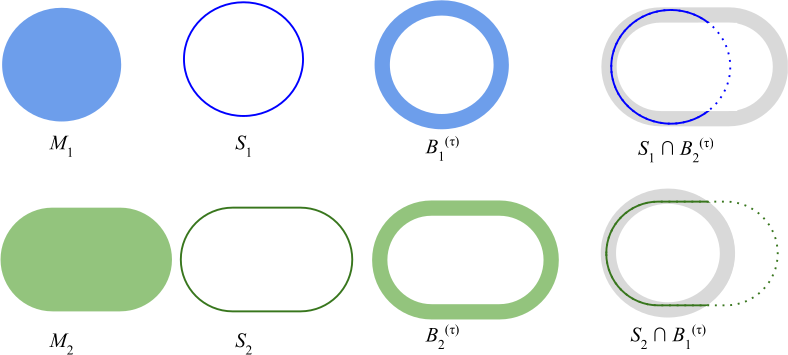
\includegraphics[width=0.85\textwidth]{sDSC}
		\caption{Illustration of equation variables seen in DeepMind's proposed surface dice similarity coefficient (sDSC), equation \ref{eq:sDSC}; and typical dice similarity coefficient (DSC), equation \ref{eq:DSC} for contours i, j. $M_{i}$ represents the volumetric mask considered in DSC measures, $B_{i}^{(\tau)}$ represents the contour surface $S_{i}$ with inter-observer variance (IOV) tolerance $\tau$, and $S_{i} \cap B_{j}^{(\tau)}$ is the intersection of surface boundaries at organ specific tolerance $\tau$: defined as the $95^{th}$ percentile absolute mean surface distance (MSD) between expert observer contours, specific to each organ considered. Figure redrawn from Nikolov et. al \cite{Nikolov_2018}.}
		\label{fig:sDSC}
	\end{center}
\end{figure}

Vaassen et. al attempted to measure the relationship between the sDSC and time required for contour correction \cite{vaassen2020}, as seen in Figure \ref{fig:vaassen}. However, this study failed to use a 95th percentile MSD for each organ-specific tolerance, as described by Nikolov et. al. Rather, a value of 1 mm was used for all organs at risk (OARs), corresponding to the x-y pixel resolution used in the study's CT scans \cite{vaassen2020}. Hence, sDSC values presented in this study are representative of variance due to spatial resolution limits and not IOV. MSD$_{95}$ values calculated from Roach et al. show organ-specific tolerances of 1.46 mm for the bladder, and 6.99 mm for the rectum. Thus, we expect sDSC values reported by Vaassen et al. to be significantly lower \cite{Nikolov_2018}, and have poorer predictive validity than when considered under correct IOV assumptions. Despite this limitation, the sDSC was a significantly better indicator of time required for correction when compared to the DSC and mean Hausdorff distance (MSHD) metrics \cite{vaassen2020}. To the best of our knowledge\todo{Unscientific language. Potentially instead say something like, `when searching through all papers indexed within PubMed that reference Nikolov et al to date, no other papers presented results regarding correlation between sDSC and correction time'}, no other attempt to correlate sDSC with correction time exists within literature.

\begin{figure}[H]
	\begin{center}
		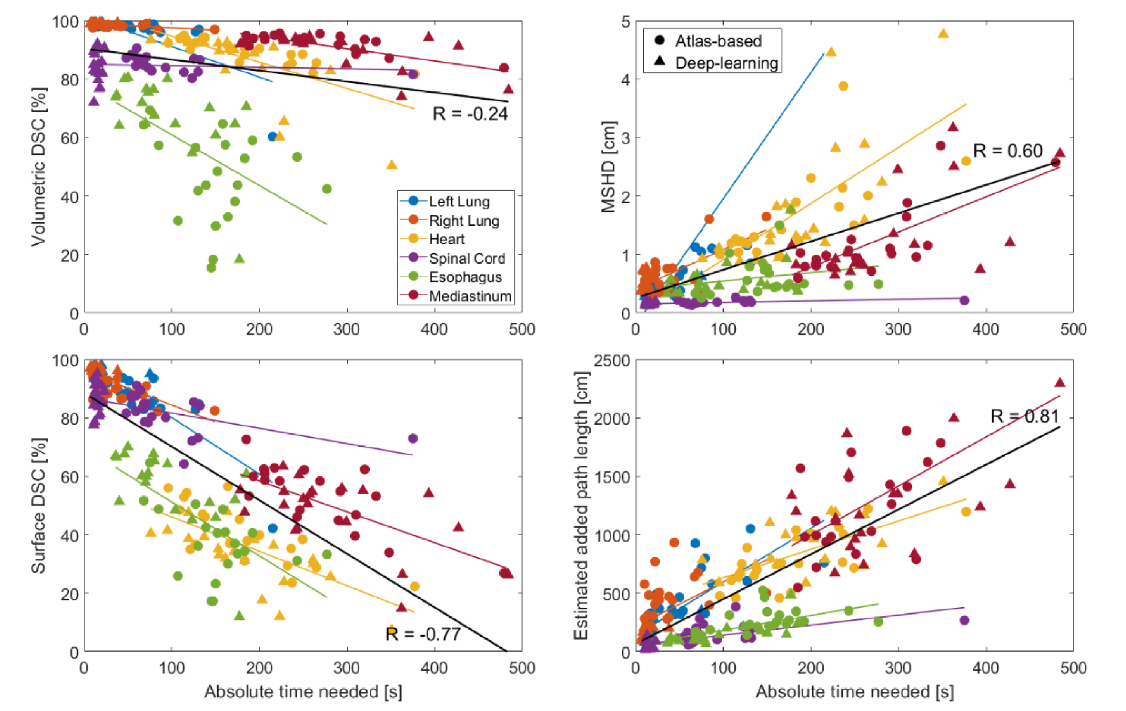
\includegraphics[width=1\textwidth]{vaassen_large}
		\caption{Vaassen et al. compare common segmentation similarity metrics with surface DSC (sDSC \cite{Nikolov_2018}) and their novel `estimated added path length' metric for ability to infer absolute time required for automatic contour correction. Atlas-based (circles) and deep-learning (triangles) methods combined. Correlation coefficients indicate a stronger relationship between sDSC value and time required, than dice similarity coefficient (DSC) and mean Hausdorff distance (MSHD) \cite{Vaassen_2020}. We note a limitation to this study is the use of an incorrect organ specific tolerance (1.0 mm - voxel size), compared to the organ specific inter-observer variance tolerance $\tau$ defined in Nikolov et. al \cite{Nikolov_2018}. Figure redrawn from Vaassen et al.  \cite{Vaassen_2020}.}
		\label{fig:vaassen}
	\end{center}
\end{figure}




%\section{Barriers to future technology: Adaptive Radiotherapy}
%U-net and CNN architecture are capable of image segmentation accuracy higher than traditional methods \cite{Ma_2019}, with much lower computational time required for inference \cite{Maier2019}


\section{Historical U-net architecture}
A 2015 study by Ronneberger et al. expanded on the concept of fully convolutional networks (FCNs by Long et al. \cite{Long2014}) to meet the challenges posed by a lack of curated training data for biomedical image segmentation \cite{Ronneberger_2015}; and to tailor FCNs for pixel-wise classification (semantic segmentation) \cite{DLINMI2018}. This breakthrough `U-net' architecture (Figure \ref{fig:unet}) includes a contracting pathway (typical of past FCNs) which downsamples resolution in the image plane to capture contextual (high-level) features for detection and general localisation \cite{Nemoto_2020}; as well as an expanding pathway, whereby high-resolution feature maps are  concatenated with matching upsampling blocks via residual skip connections \cite{Maier2019} to recover full spatial resolution in the model output \cite{DLINMI2018}. Studies report concatenating high-resolution feature maps via this secondary path improves local (detailed) feature propagation \cite{Nemoto_2020}, as later convolutions operate over both the high-resolution information provided by skip connections, and the contextual features passed via upsampling. Hence, U-net architecture facilitates multi-resolution analysis \cite{Maier2019} in an attempt to overcome the trade-off between local feature propagation and the use of contextual information in segmentation \cite{Hesamian2019}. For instance, larger kernel sizes relative to the input resolution infer spatially broader information; although, require additional pooling layers, decreasing local accuracy for detailed segmentation borders \cite{Hesamian2019}. However, studies have indicated that this trade-off still exists, as shallow U-net models tend to perform better on small segmentation regions \cite{Zhu_2018}.

Contracting (encoding) blocks were composed of two convolutional layers with 3 x 3 kernel sizing, doubling the feature channels of the input before downsampling the x-y resolution via 2 x 2 max-pooling \cite{Ronneberger_2015}. External studies have demonstrated the importance of increasing channels before max-pooling operations to avoid computational bottlenecks \cite{szegedy2015}; a strategy adopted in both paths of typical U-net models \cite{szegedy2015}. In contrast, each expanding (decoding) block upsamples resolution before halving the number of feature channels by successive  3 x 3 convolution \cite{Ronneberger_2015}. As this architecture does not make use of convolutional padding, skip connections must be cropped \cite{Ronneberger_2015}, resulting in a segmentation mask with reduced size when compared to the input image. State-of-the-art networks make use of mirrored padding to overcome this limitation \cite{Nikolov_2018}.

\subsection{Activation functions}

Activation functions present in U-net introduce non-linearity into the model, to enable learning of sophisticated features, beyond those extractable by matrix multiplication alone \cite{Maier2019}. Additionally, ReLU\todo{define this acronym?} decreases the computational burden compared to typical activation functions (such as tanh and sigmoid), whilst preserving the requirement for non-linearity \cite{Chigozie2018}. However, activation design is an ongoing area of research, with some studies noting performance improvements under modified ReLU functions (i.e. LeakyReLU) \cite{Lin2018}. Additional theory on activation functions is provided in section \ref{sec:act}.

\subsection{Data augmentation}

Pre-processing for U-net architecture routinely incorporates data augmentation, to add biologically relevant sources of variation to the training data \cite{Maier2019, Hesamian2019, Lundervold2019}. Thus, improving both model robustness and data-use efficiency \cite{Ronneberger_2015}. Dosovitskiy et al. demonstrated improved inference reliability after increasing their effective dataset size via geometric transformations, voxel intensity modulation, as well as blur and noise filters \cite{Dosovitskiy2014}. Data augmentation is also applied to balance the number of infrequent labels in a biased dataset \cite{Maier2019} - such as those in medical imaging, where relatively smaller ROIs occupy a limited volume of the total contour space \cite{Khan2019}. 


\begin{figure}
	\begin{center}
		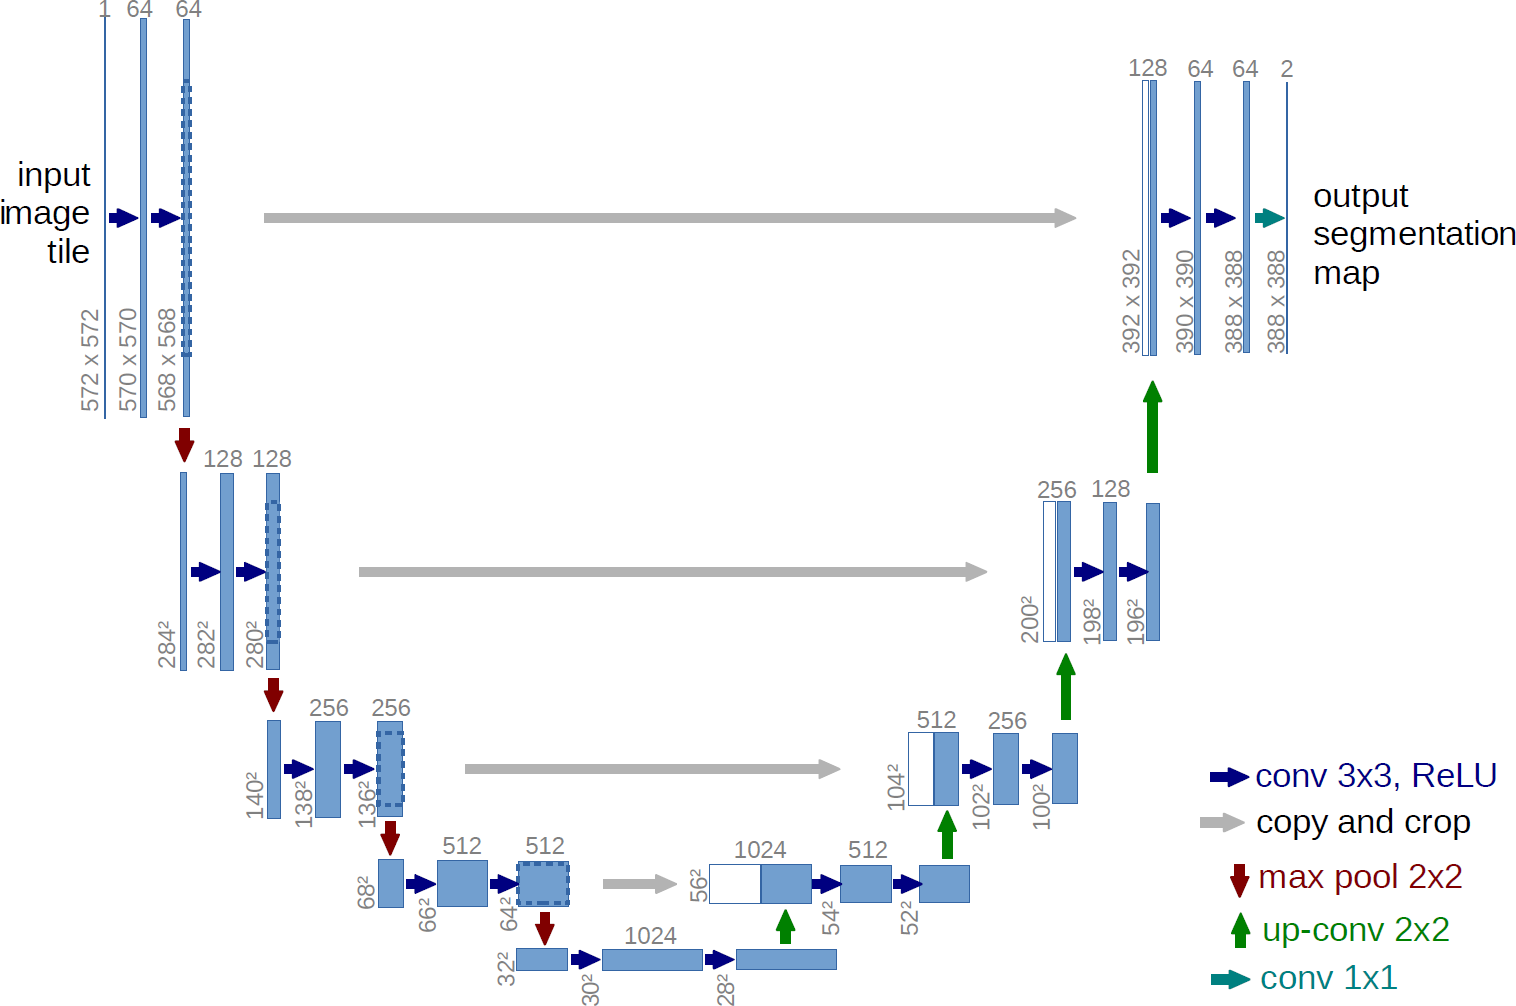
\includegraphics[width=0.9\textwidth]{ronneberger_architecture}
		\caption{Original U-net architecture first proposed in 2015 by Ronneberger et al. \cite{Ronneberger_2015}. The model consists of symmetric encoding (left) and decoding (right) pathways. Residual skip connections allow for concatenation of extracted image features at different resolutions in order to provide both high-level localisation and high resolution local information for accurate segmentation \cite{Nemoto_2020}. Figure redrawn from Ronneberger et al. \cite{Ronneberger_2015}.}
		\label{fig:unet}
	\end{center}
\end{figure}



\section{Current U-net architectures}
U-net implementations and applications vary broadly across the literature - from simplified 2D versions with 3 downsampling layers and 4 x 4 convolutions \cite{Nemoto_2020}, to 3D models that accept full patient volumes as input \cite{Zhu_2018}. A theoretical benefit of volumetric input is that organs may have axial markers that would be absent from 2D images \cite{Hesamian2019}; model inference may benefit from the richer spatial information provided by 3D inputs \cite{Nemoto_2020}. For example, Nikolov et al. presented a 3D U-net architecture for head and neck segmentation that accepted multiple context slices in addition to the primary input image \cite{Nikolov_2018} - delivering clinically acceptable contours over most datasets, for all but the smallest organs considered \cite{Nikolov_2018}. Alternative 3D implementations report promising results \cite{ Nikolov_2018, Zhu_2018, _i_ek_2016}. However, studies designed to quantify improvement over the simpler 2D architecture have shown limited performance gains \cite{Nemoto_2020}. In contrast, 3D networks require a significantly higher degree of computational resources, which may pose a challenge for clinical implementation \cite{Nemoto_2020}. In general, state-of-the-art 3D networks are trained and deployed via cloud services \cite{Nemoto_2020}; raising important ethical questions for clinics, where data is typically stored on-site with strict security and privacy protocols in place \cite{Nemoto_2020, Lundervold2019}. In addition, modified networks have experimented with feature summation between up-sampling and skip connections; however, concatenation (as in Ronneberger et al \cite{Ronneberger_2015}) has shown consistently better performance \cite{Zhu_2018}.

Nemoto et al. showed that both 2D and 3D U-net implementations were more effective than commercially available atlas-based auto segmentation tools for delineation of lung regions  \cite{Nemoto_2020}. A total of 232 patients were selected for model training and testing, with all segmentations determined manually by expert observers. In contrast to previous U-net models mentioned in this review, Nemoto et al. made use of batch normalisation layers (which aim to reduce the effect of bias output distributions from the previous layer to accelerate training \cite{santurkar2018}). Wilcoxon signed-rank testing showed that performance gains over atlas segmentation for both U-net architectures were statistically significant with $P_{val}<0.01$, and mean DSC improvement of 2.7\% \cite{Nemoto_2020}. However, no statistically significant difference was observed between 2D and 3D U-net models \cite{Nemoto_2020}, indicating that in the case of lung segmentation\todo{This is a good clarification. You are being careful here to not overstep what is being shown by the evidence. Good. Just because this organ type showed no significant improvement doesn't mean that's not true for others. Importantly, I would suspect that should an organ never be split into two sections vertically while nevertheless on some slices be hard to discern (like a gassy rectum) having superior and inferior information may inform the network that there nevertheless must be a rectum contour on the intermediate slice in question.} (a relatively large structure compared with the model output), the addition of axial input data did not translate to improved contours \cite{Nemoto_2020}.
%
%
\section{State-of-the-art models for bladder and rectum contouring}
Deep-learning segmentation has consistently shown significant improvements over traditional techniques: pixel intensity thresholding, and atlas-based image registration \cite{Cardenas2019}. In the case of pelvic imaging, poor contrast due to similar CT numbers between OARs and high variation in both location and size across patient cohorts restrict the utility of intensity and atlas-based methods \cite{acosta2013}. In addition to this, atlas approaches tend to have reduced performance in the segmentation of small volume organs \cite{acosta2013}. Ayadi et al. conducted a multi-centre prostate cancer study to evaluate the performance of a multi-atlas strategy. Expert contours were compared with Elekta's Atlas-Based Auto-segmentation (ABAS) for 26 patients, resulting in average DSC values of 0.80 $\pm$ 0.19 for the bladder, and 0.66 $\pm$ 0.09 for the rectum - requiring significant manual correction for use in RT \cite{Ayadi2011}.

In comparison, Liu et al. examined the performance of the original U-net architecture in the segmentation of pelvic OARs. Average DSC scores for CT segmentation of 105 patients were reported as 0.90 $\pm$ 0.11 and 0.78 $\pm$ 0.03 for the bladder and rectum, respectively \cite{Liu_2020}. This is comparatively lower than 2D U-net results presented by Kazemifar et al. (see Figure \ref{fig:kazemifar_unet} for schematic) who modified the original architecture via batch normalisation, increasing dropout rates, stochastic gradient descent optimisation (SGD) rather than adaptive moment optimisation (Adam), and an additional downsampling block \cite{Kazemifar_2018}. Using a DSC surrogate loss function, excellent agreement was found between observer and model contours for the 85 prostate cancer patients included in the study; with average DSCs of 0.95 $\pm$ 0.04 and 0.92 $\pm$ 0.06 for the bladder and rectum \cite{Kazemifar_2018}. In a follow-up study, Bologapal and Kazemifar et al. attempted 3D U-net architecture with an additional ResNet block (designed to improve optimisation on extremely deep networks, by minimising numerically unstable gradient flow \cite{Maier2019} i.e. the degradation problem \cite{He2015deep}), in an attempt to further improve bladder and rectum segmentation. Results showed a larger deviation between expert and model contours for the rectum, with a DSC of 0.95 $\pm$ 1.5 and 0.84 $\pm$ 3.7 for bladder and prostate, respectively \cite{Balagopal_2018}. 

\begin{figure}
	\begin{center}
		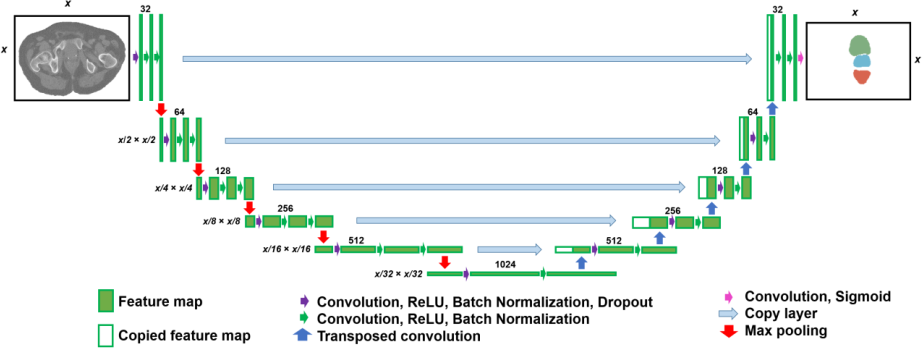
\includegraphics[width=1.05\textwidth]{kazemifar_unet}
		\caption{Modified U-net architecture used by Kazemifar et. al for state-of-the-art bladder and rectum segmentation in pelvic imaging \cite{Kazemifar_2018}. Addition of batch normalisation layers, increasing dropout rates, and additional downsampling block; when compared to the original U-net model by Ronneberger et. al. Sigmoid activation used as final layer in the network, compared with in-loss function calculation as used in Ronneberger et. al \cite{Ronneberger_2015}. Figure redrawn from Kazemifar et al. \cite{Kazemifar_2018}.}
		\label{fig:kazemifar_unet}
	\end{center}
\end{figure}

Finally, Wong et al. evaluated a commercial deep-learning package (Limbus Contour) based on U-net architecture and created an independent model for each OAR to be segmented, trained on an average of 328 CT patient scans per model \cite{Wong2020}. Specific details of the architecture are unknown due to the closed nature of the codebase \cite{Wong2020}; however, dropout and batch normalisation were selected during training \cite{Wong2020}. Data augmentation was also used, including image flipping, intensity modulation, and elastic deformations \cite{Wong2020}. Total contouring times for bladder, rectum, femoral heads, prostate, and seminal vesicles were recorded for the deep-learning model and compared to times for a single radiation oncologist (RO). The deep-learning model (DL) showed a significant time improvement (98\% reduction) over manual contouring, with an average inference of 0.4 minutes per patient (excluding manual correction), compared to 21.3 minutes for expert contour (EC) \cite{Wong2020}. In addition, DL accuracy in pelvic OAR contouring was comparable to average IOV measurements between 3 ROs \cite{Wong2020}, highlighting the clinical potential of DL contouring methods in RT. Average worst DSC (lowest DSC score for each patient scan) between DL and EC for the bladder was 0.97, with single worst case 0.95. Average worst EC-EC DSC was measured at 0.96, with single worst 0.94 \cite{Wong2020}. Rectum values showed similar consistency between DL and EC contours, with a DL-EC average worst DSC of 0.78, and single worst of 0.49. EC-EC average worst DSC of 0.79, and single worst of 0.55 \cite{Wong2020}. However, Wong et al. note the study's limitation due to a small patient testing set (20 patients per disease site) \cite{Wong2020} - small datasets are a common challenge in the application of DL methods to segmentation tasks in RT \cite{Ronneberger_2015, Maier2019, Hesamian2019, Lundervold2019}.
%

%
%
\section{Class imbalance in medical imaging}
A well-known challenge in applying deep-learning methods to medical image segmentation is the class imbalance between regions-of-interest \cite{Hesamian2019}. In particular, anatomical data in CT imaging often integrates to a much smaller volume than the background voxels, and organs inside this volume vary significantly in size \cite{taghanaki2018}. As a consequence of this input imbalance, the majority of voxels in a segmentation mask may be negatives, resulting in a a biased optimisation strategy that favours negative predictions \cite{taghanaki2018}. Multi-organ segmentation faces the additional challenge of an input class imbalance between organs, leading to parameter updates that are dominated by ROIs with the most voxels in the dataset, as these contribute most significantly to the loss calculation \cite{Khan2019}. Without accounting for this imbalance, the model can quickly become trapped in a local minimum, where optimisation occurs only for the dominant class \cite{Khan2019}. 

Output imbalance refers to a disparity between false-positive and false negative pixels in model predictions. Depending on the context, reducing false-positives may be more important than false-negatives, or vice-versa \cite{taghanaki2018}. For example by placing a higher penalty on false-positives, a model could be tailored to classify less normal tissue as a treatment volume. Conversely, penalising false-negatives may focus optimisation on difficult OARs with poor boundary contrast, reducing under-segmentation \cite{taghanaki2018}.\todo{It might be worth noting here (or maybe better done within the theory\ldots) that when utilising these tools for a QA tool it can be beneficial to provide a lower bound contour an upper bound contour and an expected average contour through having three models, one that is tuned to over-contour if it is unsure, one to under-contour if it is unsure, and the other to just give its best guess. By providing bounds the QA tool can verify if the user produced contour is within the expected bounds provided by the tool, for example, if the tool struggled to have a degree of certainty on the result it's likely not worth flagging as an incorrect contour.}

Studies indicate that the use of class weighting in loss functions can improve results by placing higher importance on contours that infrequently occur in the data, or occupy small anatomical volumes in the patient \cite{taghanaki2018}. Christ et al. showed performance gains by implementing a pixel-frequency class weighting to binary cross-entropy loss, focusing optimisation on difficult regions-of-interest \cite{ferdin2017}; and observed that accurate small lesion segmentation was not possible without class balancing, as their total contribution was less than 1\% of contour voxels \cite{ferdin2017}. In contrast, Taghanaki et al. used weighting and a combination DSC + BCE loss to enforce a desired trade-off between either false-positives or false-negatives (depending on model requirements) to correct for output imbalance; reporting improved DSC scores and lower false-negative rates for multi-organ segmentation across a range of imaging modalities \cite{taghanaki2018}. Further details of loss strategies to handle imbalance are provide in section \ref{ch:method-loss}.


% Main body: 35 - intro (1-2) - lit (6-8) = 25-28
\chapter{Theory}
\label{ch:theory}

\section{Rule 0 - No magic!}
\label{NoMagic}
Machine learning (ML) is an iterative process of improving a map between an input variable and an output target \cite{Maier2019}. In the case of medical image segmentation, initial model input corresponds to diagnostic patient images, and output to the ground truth segmentations created by an expert clinician or radiation therapist \cite{Kazemifar_2018}. More generally, the map from input to output can be interpreted as a series of pattern recognition tasks (functions) used to automate decision making \cite{Maier2019}. `Training' a model involves repeated exposure to a large representative subset of all available data, and the application of an optimisation algorithm designed to extract and select features that have predictive validity \cite{Maier2019}. For instance, if a vector $x\in\mathbb{R}^{n}$ is a complete representation of the features extracted by a model with parameters $\theta$ learned during the training phase, $\hat{y} = \hat{f}(\theta; x)$ is the prediction produced under the model $\hat{f}$.\footnote{Notation: $f(u; v)$ represents a function $f$ with variables $u$ evaluated at a fixed point $v$. For instance, in the initial input layer $v$ is the model input (CT image) upon which operators with parameters $u$ extract a feature map. This notation highlights that feature maps (also represented by $u$ when used as input in deeper layers) are dependent on the trainable model parameters $v$.} The primary decision-making unit of a neural network is the perceptron \cite{Maier2019}. Each perceptron includes a set of parameters $\theta = (w_{0}, ...,w_{n} )$, where $w_{0}$ is referred to as the activation bias, and $w = (w_{1},..,w_{n})$ as the weights. Together, these parameters perform a linear transformation $z = w \cdot x + w_{0}$ of the input $x$. A single perceptron network has the modelling capacity of a binary classifier when combined with a smooth non-linear bounded monotonic function $h$ \cite{Maier2019}; i.e. $\hat{f}(\theta; x) = h(z)$ is the perceptron output or activation value of the node (`neuron'). 


\begin{figure}[H]
	\begin{center}
		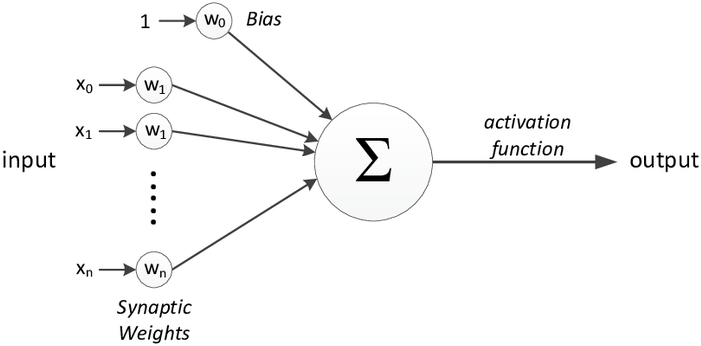
\includegraphics[width=0.7\textwidth]{perceptron}
		\caption{Single perceptron example with inputs x, trainable model parameters $\theta = (w_{0}, ...,w_{n} )$, and a non-linear activation function h. Output (or neuron activation value) is the `activated' linear combination $\hat{f}(\theta; x) = h(w \cdot x + w_{0})$. Figure adapted from Cintra et al. \cite{cintra2018}.}
		\label{fig:percept}
	\end{center}
\end{figure}
 

From here, we already have the fundamental structure required to tell a student if they would pass or fail a subject without prior knowledge of assessment weighting
(i.e. a binary classifier for pass/fail) \cite{rosenblatt1957}. For instance, by exposing the model to enough past student assessment results $x$ and their final subject score $f(x)$, parameters of the perceptron $\theta$ can converge to an approximation of the true assessment weightings \cite{Lundervold2019}. Parameter convergence is achieved via a loss function which calculates the difference between target outputs $f(x)$ under the true map $f$, and the model predictions $\hat{f}(\theta; x)$ inferred from a `forward-pass' of the learned approximation $\hat{f}$ \cite{Bertels2019}. An optimisation algorithm minimises the loss $L(\theta) \sim |f(x)-\hat{f}(\theta; x)| \to 0$ with respect to $\theta$, while ensuring changes generalise to independent cases (i.e. new student data) from a validation dataset, sampled from the same distribution as the training data (i.e. same subject) \cite{Maier2019}. We note here that $L(\theta)$ is a user defined function to measure the difference between prediction and ground truth; and that the geometric norm was presented above for simplicity. Adjustment vectors (gradients) are calculated via the familiar differential operations of calculus (as seen in equation \ref{eq:calc}) \cite{Maier2019}.
\begin{equation}
\partial_{\theta} L = \partial_{\hat{f}}  L \; \partial_{\theta} \hat{f}
\label{eq:calc}
\end{equation}

Iterative parameter updates converge $L(\theta)$ to a local minimum via a first-order approximation (equation \ref{eq:forward}), commonly referred to as the gradient descent algorithm, where $\alpha>0$ is the step-size or `learning-rate' \cite{Maier2019}.
\begin{equation}
\theta^{i+1} = \theta^{i} - \alpha \partial_{\theta} L 
\label{eq:forward}
\end{equation}

However, it is only through the combination of multiple perceptrons that we can model non-linear decision boundaries \cite{Maier2019}. Literature has shown that a single layer multi-perception network is equivalent to an XOR operator \cite{Yanling}, and hence can approximate any continuous function on a closed and bounded Euclidean subset (i.e. compact subspace) of $\mathbb{R}^{n}$ \cite{Cybenko1989}. In multi-layer (indexed from $0$ to $n$) multi-perceptron arrangements (MLPs) i.e. $\hat{f}(\theta; x)= \hat{f}_{n}(\theta_{n};(\,... \,\hat{f}_{0}(\theta_{0}; x)))$, each neuron accepts activations from the previous layer as input - facilitating the emergence of complex decision-making processes and increased modelling capacity \cite{Maier2019}. Activation functions enforce a non-linearity between model layers, preventing multi-layer networks from simplifying to linear regression models - i.e. the single perception \cite{Aggarwal2018}.  In this case, the differential vector for loss (equation \ref{eq:calc}) must account for influence through multiple network pathways via the successive application of the chain rule (i.e. the back-propagation algorithm) \cite{Maier2019}. An additional complication arises from the fact that updates are usually averaged over a subset (mini-batch) of all available training data to reduce the computational burden (via stochastic gradient descent) \cite{Sun2019}; therefore, gradient calculations occur on an approximation of the true loss topology \cite{Sun2019}. Still, all we need is calculus, linear algebra, and some additional accounting - no magic!


\section{Going deeper with convolutional neural networks}
Convolutional neural networks (CNNs) are a subcategory of MLP networks, commonly used for deep learning concerning imaging tasks \cite{Maier2019}, where we can exploit the spatial relationship of input data to reduce complexity when compared to fully connected MLPs \cite{Lundervold2019}. Typical CNN operations consist of convolutional layers that perform feature extraction \cite{Hesamian2019}; as well as pooling layers responsible for feature selection via the sub-sampling of feature maps \cite{Ronneberger_2015}. Additionally, regularisation constraints (such as dropout layers) prevent over-fitting to the training data - a state by which features extracted under the model parameters (i.e. kernels in the case of CNNs) improve performance on the training data, yet fail to generalise to independent datasets \cite{Lundervold2019}. We provide a survey of each common layer type below, with visual context provided in Figure \ref{fig:convs}.

\begin{figure}[H]
	\begin{center}
		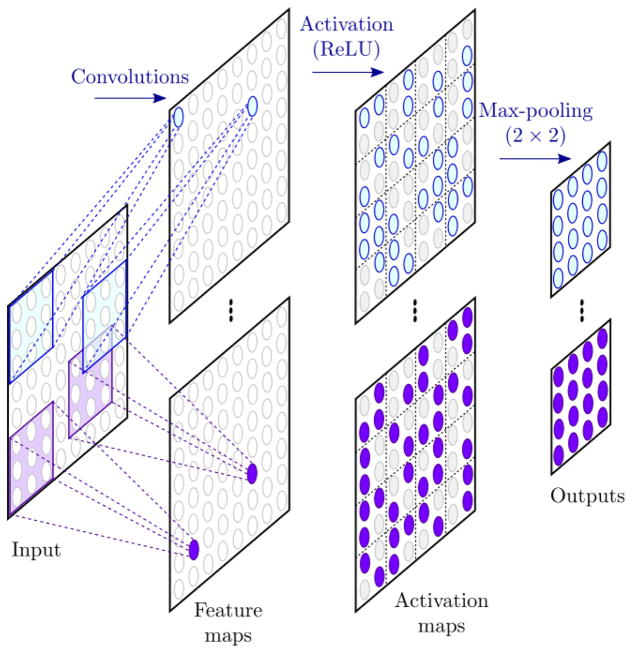
\includegraphics[width=0.65\textwidth]{convs}
		\caption{A typical sub-model arrangement seen in convolutional neural networks. Two 3 x 3 convolutional kernels (blue and purple) operate over the convolutional layer input. Each feature map has an associated kernel. The ReLU function performs non-linear activation on each extracted map. Finally, a 2 x 2 max-pooling layer halves the output dimensions and encodes a 2 x 2 translational in-variance for selected features in each partition. Figure redrawn from Hesamian et al. \cite{Hesamian2019}.}
		\label{fig:convs}
	\end{center}
\end{figure}

\subsection{Convolution layers}
Each neuron (or node) in the feature maps receives input only from a restricted subsection of the previous layer (`local connectivity'), known as the receptive field, determined by the size of the convolutional kernel \cite{Hesamian2019}. A fundamental assumption of FCNs is that spatially close input neurons (i.e. input pixel values) have an increased significance for pattern recognition when compared to distant pixels \cite{Hu2015}. For instance, a 3 x 3 kernel will convolve around activation values from the previous layer, and each node in the output feature map will have a receptive field size of 9 pixels (3 x 3) corresponding to a location in the input. In the case of CNNs, filter values in each convolutional kernel are the model parameters; optimised to extract features with predictive validity during the back-propagation phase of training \cite{Maier2019}. It follows that larger filter sizes output single node values (and hence feature maps) that are representative of a spatially broader subset of information \cite{Nemoto_2020}. Each filter in a convolutional layer is associated with a feature representation of the input (known as a feature map) \cite{Hesamian2019}. In contrast to the fully connected perceptron networks described in section \ref{NoMagic}, a single filter convolves with the same kernel weights over the entire input domain - ensuring convolutional in-variance across an individual feature map \cite{Maier2019} - hence a specific pattern recognition task can be associated with each kernel in the layer \cite{Zeiler_2014}. In addition to making sense conceptually (i.e. edge detection is likely as useful over the entire input as it is on a kernel-sized subset), this `parameter sharing' has the added advantage of significantly reducing the total number of parameters in a model; reducing both computational complexity and GPU memory requirements - allowing for deeper learning \cite{Lundervold2019}.

\subsection{Pooling layers}
Pooling is a technique for sub-sampling feature maps in order to decrease resolution; and, to encode translational in-variance to activation values in its receptive field \cite{Lundervold2019}. For instance, a 2 x 2 max-pooling layer outputs the maximum value from each non-overlapping 2 x 2 grid partitioned from its input, halving the total feature map dimensions in the x-y plane, and encoding spatial in-variance with respect to the selected value over the 2 x 2 grid \cite{Lundervold2019}. Downsampling in this way is also possible via a 2D convolution with a stride size of 2. Convolutional pooling adds trainable parameters in the form of a kernel and has the benefit of simplifying the overall network structure due to the linear nature of convolution \cite{springenberg2014}.

\subsection{Dropout layers}
Dropout layers enforce a regularisation constraint by randomly sampling neurons in a network for deactivation; enforcing redundancy in a network, as adjusted architectures process each training batch \cite{Lundervold2019}. Weights are therefore optimised on multiple sub-variations of the complete network, resulting in stochastic averages with values sampled from a broad ensemble of networks \cite{srivastava2014}. Dropout layers improve generalisation and hence model performance when compared to fixed architectures. We note that dropout is deactivated during post-training inference, and predictions occur via the complete architecture \cite{Lundervold2019}.

\begin{figure}[H]
	\begin{center}
		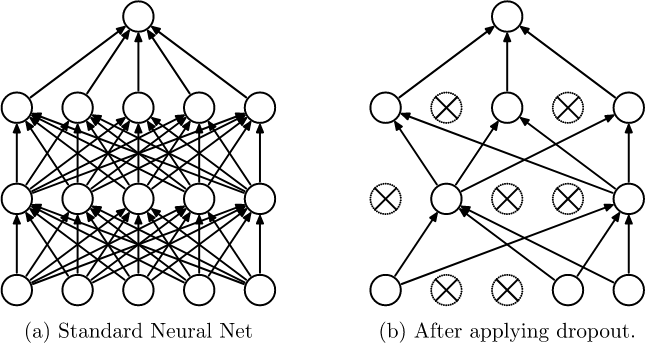
\includegraphics[width=0.65\textwidth]{dropout}
		\caption{Multi-layer perceptron with 2 hidden layers. (a) Standard network without dropout applied. (b) Standard network after applying dropout. The dropout technique randomly samples neurons in the network for deactivation, allowing parameter tuning to occur as averages over an ensemble of networks. Figure redrawn from Srivastava et al. \cite{srivastava2014}.}
		\label{fig:dropout}
	\end{center}
\end{figure}

\subsection{Batch normalisation layers}
Batch normalisation layers are typically placed after activation layers (ordering is a topic of current research and alternative variations exist i.e. \cite{Kazemifar_2018}) to normalise activated feature maps. Hence, each batch normalisation layer adds two trainable parameters to the model, a mean and a variance value \cite{Lundervold2019}. Although batch normalisation has been shown to accelerate training and improve stability in layer distributions, its effectiveness is poorly understood from a theoretical perspective \cite{santurkar2018}. Conventional understanding states that batch normalisation penalises internal co-variance between network layers \cite{ioffe2015} and reduces effects of the vanishing/exploding gradient problems \cite{Li2014}. Additionally, parameter updates to feature maps in earlier layers are likely to significantly change the feature distribution of deeper layers - compounding internal variance in the optimisation process \cite{santurkar2018}. Hence, by normalising the output activation map, changes in layer distributions can be stabilised \cite{santurkar2018}. Conversely, studies have reported minimum improvements to internal co-variance under batch normalisation; and report that performance improvement is due to a smoothing of loss topology, which stabilises the behaviour of gradient descent \cite{santurkar2018}.

\subsection{Activation functions}
\label{sec:act}
In the previous section, we presented the fundamental structure of MLPs and expanded on this by examining CNN layers. However, `deep' learning is not possible with the typical sigmoid activation function presented in early MLP networks \cite{Lundervold2019} (included in equation \ref{eq:sigmoid}) due to the vanishing gradient problem - whereby multiple derivatives in the back-propagation algorithm with values $<1$ cause the loss gradient (equation \ref{eq:calc}) to decay exponentially as a function of the number of layers \cite{Lundervold2019}. 
\begin{equation}
\sigma(x) = \frac{1}{1+e^{-x}}
\label{eq:sigmoid}
\end{equation}

In contrast, convex functions such as the piecewise linear ReLU (Rectified linear unit - equation \ref{eq:ReLU}) have shown improved performance in deep layer arrangements due to the sparse nature of their activation \cite{Krizhevsky2012}; and, as non-saturating gradients prevent the vanishing gradient problem \cite{Lundervold2019}. However, contrary to activation function requirements stated in section \ref{NoMagic}, ReLU is neither smooth nor bounded, raising some technical challenges in its use \cite{Lundervold2019}. The unbounded nature of ReLU exposes the network to the well-known `exploding gradient problem' - as there is no constraint on activation values \cite{xu2015}. In addition, the `Dying ReLU problem` highlights a limitation associated with zeroing all negative activation inputs \cite{xu2015}. Zeroed activation values may fail to influence the loss function during gradient calculations; hence, this state partially prohibits parameter adjustment during training \cite{xu2015}. Although some recent CNN implementations attempt to offset the Dying ReLU problem via the so-called `Leaky ReLU' (which maintains a small non-zero gradient for activations $< 0$ \cite{Maas2013}), ReLU is still the default recommendation for most deep neural networks \cite{Goodfellow2016}.

\begin{equation}
ReLU(x) = max(0,x)
\label{eq:ReLU}
\end{equation}


\section{Loss functions}

%Calculations for weighted soft DSC were performed via equation \ref{eq:method_wsdsc}, with component equations presented in \ref{eq:w}, \ref{eq:i}, and \ref{eq:u}. $W$, $I$, and $U$ correspond to the weight, intersection and union vectors, indexed with respect to each contour structure by $k\in\{1,...,n\}$; while $\epsilon$ represents a small value $>0$ to ensure division is defined. In addition, $|\cdot|$ notation refers to the cardinality of a set (i.e. the total number of pixels in a contour mask - including zeros), while $t_{k}$ refers to a ground truth array, $p_{k}$ to the predicted array, and $\odot$ to the Hadamard product. The standard soft DSC can be implemented by setting weights $W=\vec{1}$.  Code required for a TensorFlow implementation is included in the PyMedPhys library.

%\begin{equation}
%\textrm{w. soft DSC} = \frac{2 \, (W \cdot I + \epsilon)}{W \cdot U + \epsilon}
%\label{eq:method_wsdsc}
%\end{equation}

%\todo{Is it appropriate to include a footnote with link to a specific commit hash (so future moving of stuff doesn't break the link), for example https://github.com/pymedphys/pymedphys/tree/9ef43ae/examples/protyping/pymedphys-segmentation}

%\begin{equation}
%\textrm{w. soft DSC} = \frac{2 \, (W \cdot I + \epsilon)}{W \cdot U + \epsilon}
%\label{eq:method_wsdsc}
%\end{equation}
%
%\begin{equation}
%W = (W_{1}, ..., W_{n}) \; \; \textbf{:} \; \; W_{k} = \frac{\sum_{k=1}^{n} |t_{k} |}{t_{k} + \epsilon}
%\label{eq:w}
%\end{equation}
%
%\begin{equation}
%%I = (I_{1}, ..., I_{n}) \; \; \textbf{:} \; \; I_{i} = \langle\,t_{i} \,,\,  p_{i}\,\rangle
%I = (I_{1}, ..., I_{n}) \; \; \textbf{:} \; \; I_{k} = \sum_{i,j=1}(t_{k} \, \odot \,  p_{k})_{ij}
%\label{eq:i}
%\end{equation}
%
%\begin{equation}
%U = (U_{1}, ..., U_{n}) \; \; \textbf{:} \; \; U_{k} =  \sum_{i,j=1}(t_{k} + p_{k})_{ij}
%\label{eq:u}
%\end{equation}
%
%\todo[inline, color=blue!40]{Addition? - Tversky loss formula and parameters used - \cite{abraham2018}}
\begin{equation}
\textrm{BCE} = -\frac{1}{N}\sum_{n=1}^{N}r_{n} \; log(p_{n}) \; + \; (1-r_{n}) \; log(1-p_{n})
\label{eq:method_bce}
\end{equation}


\begin{equation}
\textrm{w. soft DSC$_{loss}$} = 1-2\frac{\sum_{l=1}^{2}w_{l}\sum_{n}r_{ln}p_{ln} + \epsilon}{\sum_{l=1}^{2}w_{l}\sum_{n}r_{ln} + p_{ln} + \epsilon} \; \;  \; \; \textbf{:} \; \; \; \; w_{l} = \frac{1}{\sum_{n=1}^{N}(r_{ln} + \epsilon)^2}
\label{eq:method_wsdsc}
\end{equation}
%
soft DSC loss can be recovered by setting $w_{l}$ = $\vec{1}$

The Tversky index (seen in \ref{eq:method_TI}) is an extension of the soft DSC loss designed to enforce a trade-off between false-positives and false-negatives via the tuning of the $\alpha$ and $\beta$ parameters \cite{Khan2019}. For example, DSC is the harmonic mean of recall (sensitivity) and precision, and places equal eighting on false positives and false negatives. This can be recovred in the Tversky index by setting $\alpha = \beta = 0.5$

\begin{equation}
\textrm{T}(\alpha, \beta) = \frac{\sum_{l=1}^{2}r_{ln}p_{ln} + \epsilon}{
\sum_{l=1}^{2}r_{ln}p_{ln} +
\alpha\sum_{l=1}^{2}r_{l\bar{n}}p_{ln} +
\beta\sum_{l=1}^{2}r_{ln}p_{l\bar{n}} + \epsilon	
}
\label{eq:method_TI}
\end{equation}

The focal Tversly loss is an extension of the focal cross entropy loss presented by Lin to 

\begin{equation}
\textrm{FTL}(\alpha, \beta) = \sum(1-\textrm{TL}(\alpha, \beta))^{1 / \gamma}
\label{eq:method_TL}
\end{equation}

\chapter{Method}
\label{ch:method}

\section{Datasets}
\label{ch:method-dataset}
This project focused on building an automated segmentation solution for radiotherapy. Two applications were targeted: A multi-organ segmentation model for pelvic imaging (with patient, bladder and rectum contouring); and a single structure model for vacuum bag contouring in canine imaging.\todo{maybe here add `as described in section blah'} Anonymised pelvic imaging data was provided by Riverina Cancer Care Centre from active prostate cancer RT patients over multiple stages of treatment. Canine imaging data was provided by the Small Animal Specialists Hospital (SASH) and contained variable cancer locations and patient orientations. All input data consisted of raw diagnostic CT images acquired with a 512 x 512 matrix. Pelvic imaging scans were comprised of 1.37 mm x 1.37 mm x 2 mm voxels; while canine imaging scans contained variable spacings across patients, with an average voxel size of 0.85 mm x 0.85 mm x 1.907 mm\todo{probably better to just use one decimal place here}.

Patient scans were converted from a propriety Monaco format (.WC files)
\todo{Did you actually do this? Or do you mean instead ``plans were exported from the TPS in DICOM format''?}
to DICOM files, from which image-structure pairs were extracted, transformed from patient-space to a non-dimensional matrix-space, and saved individually as model input-output arrays for further processing. Initial modelling was attempted with contours extracted on-the-fly from DICOM files; however, this resulted in a significant CPU bottleneck which limited GPU capacity during training.
\todo{This could have been fixed by caching your transformations to disk and subsequently to memory. You have essentially implemented this, it's just that if it was in the cache model philosophy the model would see a DICOM file, check to see if it exist in memory, if not, check to see if it has a numpy conversion of it saved to disk, if not, then it would do the conversion, save the numpy result to disk, and store it in memory. Next time that file is needed, it would find in memory, or if you shutdown the software it'll find it saved to disk. In its current format you've essentially implemented a manual cache without supporting the original format.}
In addition, any advantage of removing the intermediate file processing step (DICOM to array) was made redundant upon determining that significant data cleaning would be required for contour consistency. For instance, vacuum bag segmentation was often incomplete in patient scans, as only clinically relevant locations included full contouring; this may satisfy clinical requirements, however, consistent labels are required for machine learning. The final data pipeline was designed to handle filenames (pointing to arrays) as the primary method of matching an input with the ground truth. From here, an array for each filename was read into memory if it belonged to the current batch; this removed memory constraints on dataset size as only a single batch populated the RAM at each training step.

A total of 15 patients were used for pelvic imaging, corresponding to 1991 total input instances. Data was split at the patient level to enforce independence across training, validation and test datasets. 12 patient scans were used for training, while validation and testing used 2 and 1, respectively. The complete data distribution is provided in Table \ref{table:data_prostate}. Patient contours were present in all input data, while the bladder was present in 28\% of slices, and rectum in 37\%. We note the significant pixel-wise class imbalance between structures, as the output space was 512 x 512 x 3 for multi-organ segmentation. Patient pixels corresponded to a total of 5.21\% of all output pixel in the data, with 0.081\% and 0.021\% corresponding to bladder and rectum.

\begin{table}[H]
\footnotesize
\caption{Data distribution for pelvic imaging.}
\centering
\begin{tabular}{c c c c c}
\hline\hline
& Training & Validation & Testing & Total  \\ [0.5ex]
\hline

Images(Patients) & 1751(12) & 282(2) & 138(1) & 1991(15) \\
 \\
 \hline\hline
		 & Images total (\%) & Pixel-image ratio (\%)& Pixel-output ratio (\%) & Pixels total (\%)\\ [0.5ex]
\hline
Patient  & 100 & 15.6  &  5.21 & 5.21\\
Bladder  & 28.0 & 0.862 & 0.287 & 0.081\\
Rectum   & 37.0 & 0.172 & 0.057 & 0.021\\
\hline\hline
\end{tabular}
\label{table:data_prostate}
\end{table}


For vacuum bag segmentation, a total of 26 patients were used, with 21, 3, and 2 corresponding to training, validation and testing, respectively. Vacuum bag structures were present in 70\% of total input images, as seen in Table \ref{table:data_vet}.

\begin{table}[H]
\footnotesize
\caption{Data distribution for canine imaging.}
\centering
\begin{tabular}{c c c c c}
\hline\hline
& Training & Validation & Testing & Total  \\ [0.5ex]
\hline

Images(Patients) & 1912(21) & 340(3) & 187(2) & 2439(26) \\
 \\
 \hline\hline
		 & Images total (\%) & Pixel-image ratio (\%)& Pixel-output ratio (\%) & Pixels total (\%)\\ [0.5ex]
\hline
Vacbag   & 70.0& 13.4  & 13.4  &  9.4 \\

\hline\hline
\end{tabular}
\label{table:data_vet}
\end{table}



Significant data augmentation was used to increase the effective size of our dataset and to regularise over-fitting. Augmentation was performed on-demand for each input-output pair in a batch, and sampled from a random uniform distribution with probability listed below for each type. 50\% of total training data was selected for augmentation per epoch. Augmentations included: Left-right image inversion ($P_{val}=0.5$), random image cropping and resizing ($P_{val}=0.33$, minimum crop size 500 x 500), elastic deformations ($P_{val}=0.33$, with ($\alpha$, $\sigma$) pairs selected from (1201, 10), (1501, 12), and (991, 8)), affine transformations ($P_{val}=0.33$, $\alpha_{max}=20$), and Gaussian noise ($P_{val}=0.33$, $\mu=0$, $\sigma_{max}=0.3$). Furthermore, all input data (including test data) was normalised with respect to the training and validation dataset distributions prior to augmentation. Randomly sampled transformations are included in Figure \ref{fig:augment}.

\begin{figure}[!htb]
	\begin{center}
		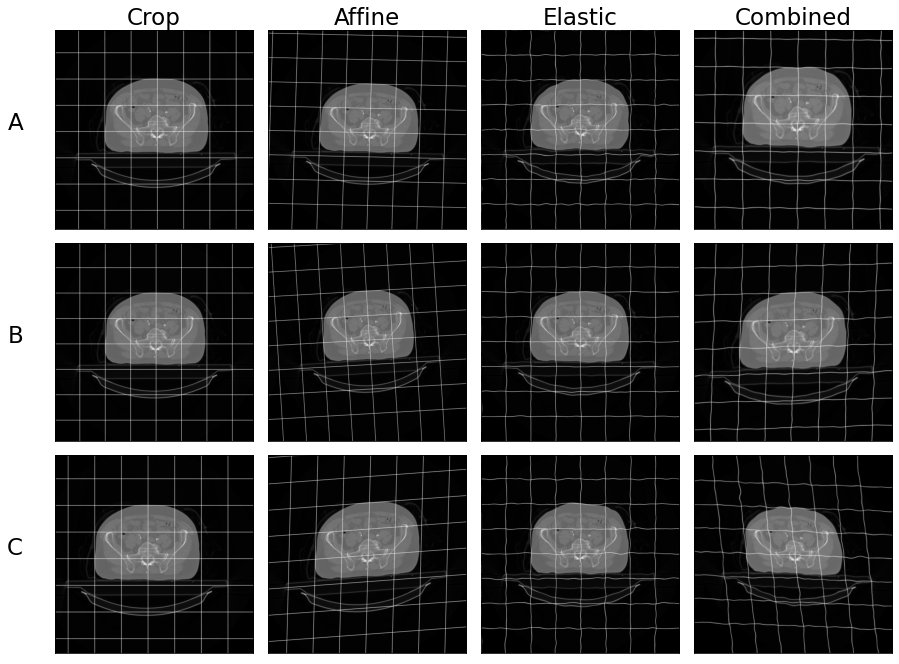
\includegraphics[width=1\textwidth]{figures/augment}
		\caption{Training data augmentation for single input image with random sampling of parameters: image crop and resize, affine transformation, elastic deformation, and combined transformations. Each matching contour set is augmented under an identical transformation. An individual transformation type has $P_{val}=0.33$ of occurring. Additional augmentations not shown: Left/right inversion and Gaussian noise}
		\label{fig:augment}
	\end{center}
\end{figure}

\section{Model architecture}
\label{ch:method-architecture}
We designed a 2D U-net architecture with 7 levels, consisting of 6 encoding and 6 decoding blocks, outlined in Figure \ref{fig:model}. The model accepts a full resolution (512 x 512) CT image as input, and outputs selected contours in the original resolution by the use of padded convolutions, each of which is followed by batch normalisation and ReLU activation. Each encoding block performs a repeated sequence of 3 x 3 convolution (increasing feature channels). Extracted feature maps are passed via the skip connection in one pathway, while a 3 x 3 convolution with stride size 2 halves the resolution before passing features to the next encoding block.

Conversely, each decoding block upsamples input via a 3 x 3 2D transposed convolution with stride size of 2. Upsampled feature maps are then concatenated with skip connections. Dropout is selectively performed with a probability value of 20\%, before additional 3 x 3 convolution sequences reduce the feature channels.

Finally, multi-organ segmentation can be controlled via the C (Channel - corresponding to the number of segmentations) output variable specified in the last 1 x 1 convolutional layer. A sigmoid activation function is used to account for the non-mutually exclusive nature of pixel-wise binary classification on anatomic structures (i.e. a voxel can belong to multiple structures).

\begin{figure}[!htb]
	\begin{center}
		\hspace*{-1.3cm}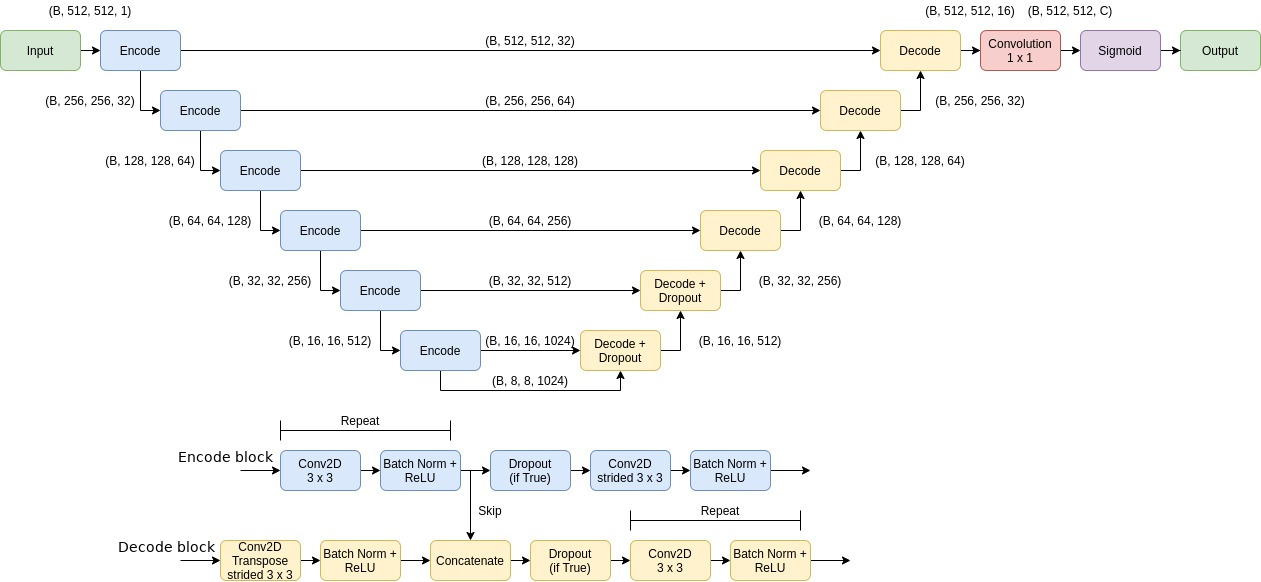
\includegraphics[width=1.15\textwidth]{figures/model_diagram}
		\caption{Modified 2D U-net architecture: Composed of encoding (blue) and decoding blocks (yellow). MaxPooling layers replaced by strided convolution. Added batch normalisation and final sigmoid activation.Tensor dimensions (Batch size, X, Y, Channels) are included for each connection. Internal layers of encoding blocks (blue) and decoding blocks (yellow) are included under the high-level overview.}
		\label{fig:model}
	\end{center}
\end{figure}

The model was trained using the Adam (Adaptive momentum estimation) optimisation algorithm \cite{kingma2014} with an initial learning rate of $10^{-5}$, a batch size of 1 for pelvic imaging, and 3 for canine imaging. Model training was scheduled to conclude when validation loss had not improved for a period of 20 epochs. In addition, learning rate decay was triggered by a validation loss plateau period of 3 epochs. Initial model weights were determined via `He' kernel initialisation), which samples from a zero mean Gaussian distribution with variance $\sigma=\sqrt{2/N}$ (as in Ronneberger et al \cite{Ronneberger_2015}), where N is the incoming nodes for a single activation (i.e. for n x n convolution over M feature maps, N = n x n x M). In addition, we accelerate training for pelvic imaging by adopting the strategy of Bertels et. al to further initialising model parameters via 3 epochs of training with binary cross entropy.



\section{Loss functions}
\label{ch:method-loss}
A total of 5 loss functions were assessed for pelvic imaging: Binary Cross entropy (BCE), soft dice similarity coefficient (soft DSC) \cite{Bertels2019}, weighted soft dice similarity coefficient (w. soft DSC or modified generalised dice loss \cite{Sudre_2017}), a modified combination loss BCE + 2 (w. soft DSC) \cite{taghanaki2018}, and focal Tversky loss \cite{Zhu_2018, Khan2019, abraham2018}. In contrast, weighted soft DSC was not attempted for canine imaging due to the single segmentation output.

Calculations for weighted soft DSC were performed via equation \ref{eq:method_wsdsc}, with component equations presented in \ref{eq:w}, \ref{eq:i}, and \ref{eq:u}. $W$, $I$, and $U$ correspond to the weight, intersection and union vectors, indexed with respect to each contour structure by $k\in\{1,...,n\}$; while $\epsilon$ represents a small value $>0$ to ensure division is defined. In addition, $|\cdot|$ notation refers to the cardinality of a set (i.e. the total number of pixels in a contour mask - including zeros), while $t_{k}$ refers to a ground truth array, $p_{k}$ to the predicted array, and $\odot$ to the Hadamard product. The standard soft DSC can be implemented by setting weights $W=\vec{1}$.  Code required for a tensorflow implementation is included in the pymedphys library.

\begin{equation}
w. \, soft \, DSC = \frac{2 \, (W \cdot I + \epsilon)}{W \cdot U + \epsilon}
\label{eq:method_wsdsc}
\end{equation}

\begin{equation}
W = (W_{1}, ..., W_{n}) \; \; \textbf{:} \; \; W_{k} = \frac{\sum_{k=1}^{n} |t_{k} |}{t_{k} + \epsilon}
\label{eq:w}
\end{equation}

\begin{equation}
%I = (I_{1}, ..., I_{n}) \; \; \textbf{:} \; \; I_{i} = \langle\,t_{i} \,,\,  p_{i}\,\rangle
I = (I_{1}, ..., I_{n}) \; \; \textbf{:} \; \; I_{k} = \sum_{i,j=1}(t_{k} \, \odot \,  p_{k})_{ij}
\label{eq:i}
\end{equation}

\begin{equation}
U = (U_{1}, ..., U_{n}) \; \; \textbf{:} \; \; U_{k} =  \sum_{i,j=1}(t_{k} + p_{k})_{ij}
\label{eq:u}
\end{equation}

\todo[inline, color=blue!40]{Addition? - Tversky loss formula and parameters used - \cite{abraham2018}}

Final model performance was evaluated on an independent test dataset via both DSC and sDSC metrics. Organ specific tolerance $\tau$ for rectum and bladder contours were taken as the 95th percentile absolute mean surface distance in mm between expert observers from Roach et al. \cite{Roach_2019}. MSD$_{95}$ values calculated from Roach et al. show organ-specific tolerances of 1.46 mm for the bladder, and 6.99 mm for the rectum.
\chapter{Results and discussion}
\label{ch:results}
\todo{Results and Discussion}

\section{Model 1: Pelvic imaging}
A total of 5 loss functions were assessed for ability to train a 2D U-net with a small dataset. As seen in Table \ref{table:loss_prostate}, dice similarity coefficient (DSC), precision and sensitivity metrics were recorded on an independent test dataset to measure model generalisability for each loss. Binary cross entropy (BCE) is a pixel-wise similarity measure \cite{Bertels2019},
\todo{You shouldn't need to be explaining anything to me about BCE in your results section.}
and achieved the strongest scores with a DSC of 0.996, precision of 0.999, and sensitivity of 0.991. Patient contouring under BCE was excellent,
\todo{No need to add in subjective language, the numbers speak for themselves. There's no place for subjective language in this kind of report. If you want to make a statement of quality say something like ``Every predicted contour on every slice were within range of IOV found within the literature'' or something to that tune, as long as you have those numbers, and it's true of course. Express quality by stating it is above a well defined threshold, ideally a threshold for quality that you've defined within your theory section.}
with an average organ specific DSC of 0.996; however, BCE failed to produce any positive predictions for the rectum, and only large bladder examples were identified - likely due to the built-in assumption that classes are balanced \cite{Ronneberger_2015}. Reports have indicated that BCE has sub-optimal performance on class imbalanced data \cite{taghanaki2018}; however, large bladder examples were contoured accurately
\todo{`accurately' what do you mean? Maybe something like ``bladder examples were contoured within the IOV for that organ''.}
(see Figure \ref{fig:prostate_BCE_bladder}).  

The standard soft DSC loss function also assumes equally weighted segmentation classes throughout the data \cite{Sudre_2017}; and hence, failed to produce positive predictions for the bladder and rectum. However, patient contouring was again excellent, with mean DSC 0.996. Research has indicated that the DSC is equivalent to the harmonic mean of recall (sensitivity) and precision \cite{Bebis2019}; and hence, weighs both equally \cite{Bebis2019} - contributing to the class imbalance problem as the majority of output pixels are negatives. It is not possible to control the trade-off between false-positives and false-negatives in the standard soft DSC loss formulation \cite{taghanaki2018}; as expected, we observe a bias that favours negatives due to their over-representation in model output \cite{taghanaki2018}.  To control for class imbalance in pelvic CT imaging (where boundaries between OARs can be poorly defined) we likely require a loss function that enforces a higher penalty for false-negative values, such that target regions are not under-segmented \cite{taghanaki2018}. An additional point of warning to note is that the soft DSC does not include true-negatives in its calculation, hence specificity is not optimised directly \cite{taghanaki2018}.

 Conversely, the weighted soft DSC loss function (presented in equation \ref{eq:method_wsdsc}) was the only loss attempted that was able to optimise for all organs in the contour space (see Figures \ref{fig:prostate_patient}, \ref{fig:prostate_bladder}, and \ref{fig:prostate_rectum}), and was selected as our final model loss. We note that a simplified combination BCE and weighted soft DSC loss was also attempted (see \cite{taghanaki2018}) after experiments revealed BCE performance was superior to the standard soft DSC metric, and contoured larger bladder examples more accurately than the weighted soft DSC. However, only patient contours were produced - reinforcing that scalar selection to optimally balance a linear combination of loss functions is a non-trivial task dependent on the data distribution \cite{Bertels2019}. 
 
 Focal Tversky loss (see \cite{Khan2019}) exceeded both BCE and the combination loss in sensitivity; however, performed poorly on average volumetric overlap (DSC). Tversky loss successfully identified rectum and bladder contours in almost all cases; however, segmentation masks contained many false-positive results, with additional groupings that neither resembled nor were spatially close to the OAR in question. We note that although Tversky loss aims to improve the trade-off between sensitivity and precision compared to DSC for highly imbalanced data (i.e. by weighting to penalise false-negatives higher than false-positives) \cite{taghanaki2018}; our results in Table \ref{table:loss_prostate} indicated sensitivity was lower when compared to BCE and the weighted soft DSC loss. However, Focal Tversky was the only loss function to perform higher in sensitivity than precision - consistent with a higher weighting on false-negatives as described in the literature \cite{Khan2019}.

\begin{table}[H]
\footnotesize
\caption{Loss evaluation on independent test dataset for pelvic imaging}
% title of Table
\centering
% used for centering table
\begin{tabular}{c c c c}
% centered columns (4 columns)
\hline\hline
%inserts double horizontal lines
Loss & DSC & Precision & Sensitivity \\ [0.5ex]
% inserts table
%heading
\hline
% inserts single horizontal line
BinaryCrossentropy (BCE) & 0.995 & 0.999 & 0.991 \\
soft DSC & 0.986 & 0.999 & 0.972 \\
\textbf{w. soft DSC} & \textbf{0.994} & \textbf{0.997} & \textbf{0.991} \\
BCE + 2(w. soft DSC) & 0.985 & 0.999 & 0.971 \\
FocalTversky & 0.962 & 0.941 & 0.987 \\
% [1ex] adds vertical space
\hline\hline
%inserts single line
\end{tabular}
\label{table:loss_prostate}
% is used to refer this table in the text
\end{table}


Our final model for pelvic imaging was selected at the 140th epoch, under weighted soft DSC. As seen in Figure \ref{fig:prostate_metrics}, validation loss plateaued at 130 epochs, with DSC value reaching a maximum at 140 epochs. We note that although a smoothed representation of loss for both validation and training data would be monotonically decreasing, this is not the case for DSC, precision, and sensitivity metrics. In section \ref{ch:method-architecture} we noted the use of BCE weight initialisation; after switching from BCE to weighted soft DSC, there is a significant change in loss topology. Examination of early model predictions after BCE initialisation indicated a change in state from placing minimal significance on bladder and rectum cases, to now having gradients dominated by changes to these organs under weighted soft DSC. It is likely that feature representation were subsequently perturbed significantly to minimise the new loss - temporarily decreasing DSC and precision. A similar pattern emerged for DSC value under Focal Tversky; however, the initial DSC value is comparatively lower than under weighted soft DSC - indicating that convergence after 3 epochs of BCE is likely sensitive to randomly sampled weight initialisation \cite{Ronneberger_2015}. Total inference time per patient was approximately 3 seconds.

\begin{figure}[H]
	\begin{center}
		\hspace*{-1.2cm}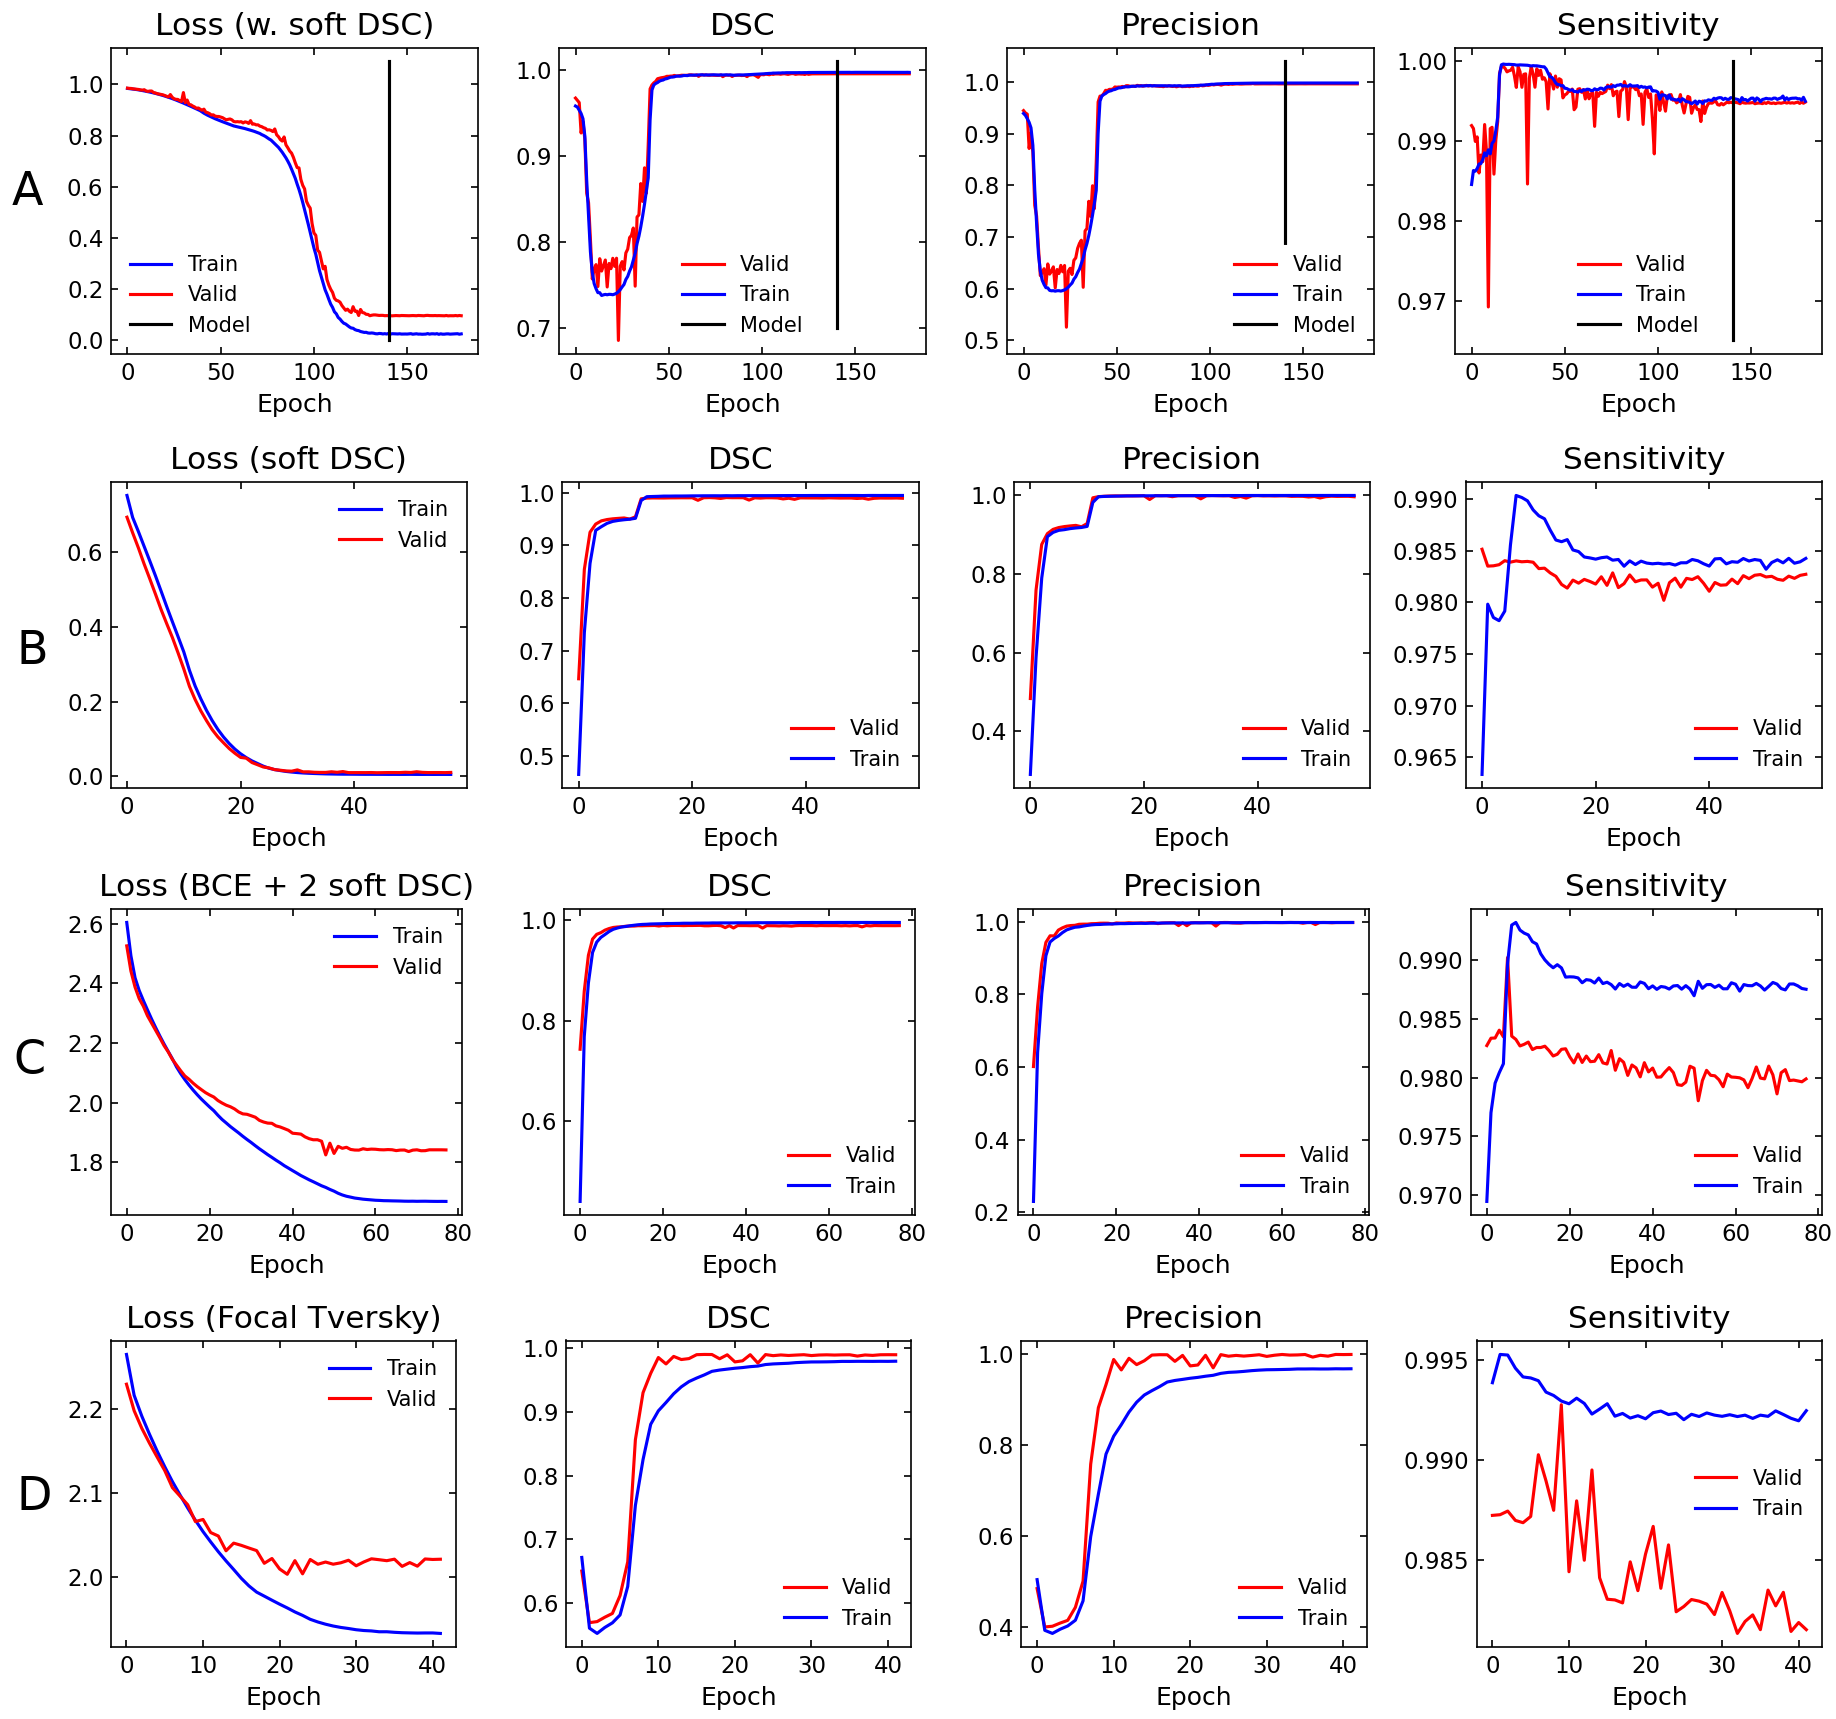
\includegraphics[width=1.15\textwidth]{figures/prostate_metrics_all}
		\caption{\textbf{A)} Model training metrics for pelvic imaging via weighted soft DSC loss (w. soft DSC). Final model selected at epoch 140 due to validation loss plateau. Metrics begin post binary cross entropy (BCE) weight initialisation (3 epochs). Training time of 9 hours. \\
		\textbf{B)} Soft dice similarity coefficient (soft DSC) loss \\
		\textbf{C)} Combination binary cross entropy (BCE) and weighted soft dice similarity coefficient (w. soft DSC) loss\\
		\textbf{D)}  Focal Tversky loss}
		\label{fig:prostate_metrics}
	\end{center}
\end{figure}


\begin{figure}[H]
	\begin{center}
		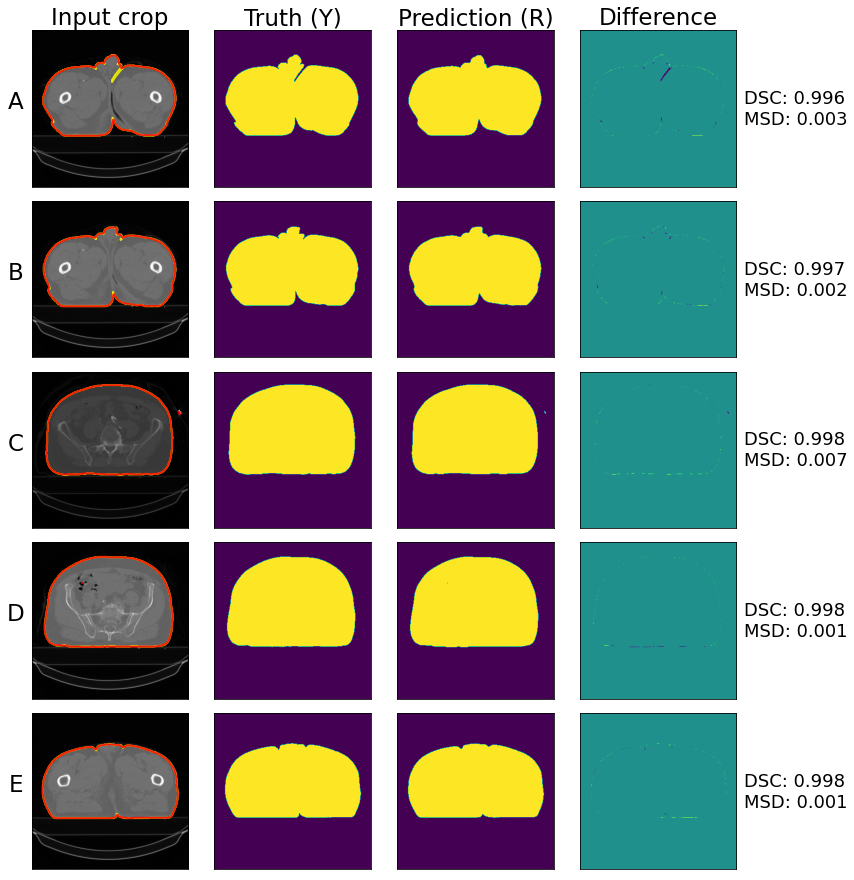
\includegraphics[width=1.0\textwidth]{figures/prostate_patient}
		\caption{Representative output for patient. Model 1 - trained via weighted soft dice (w. soft DSC) loss - 140 epochs.  Truth contour (yellow), prediction contour (red). Mean surface distance (MSD) mm.}
		\label{fig:prostate_patient}
	\end{center}
\end{figure}



\begin{figure}[H]
	\begin{center}
		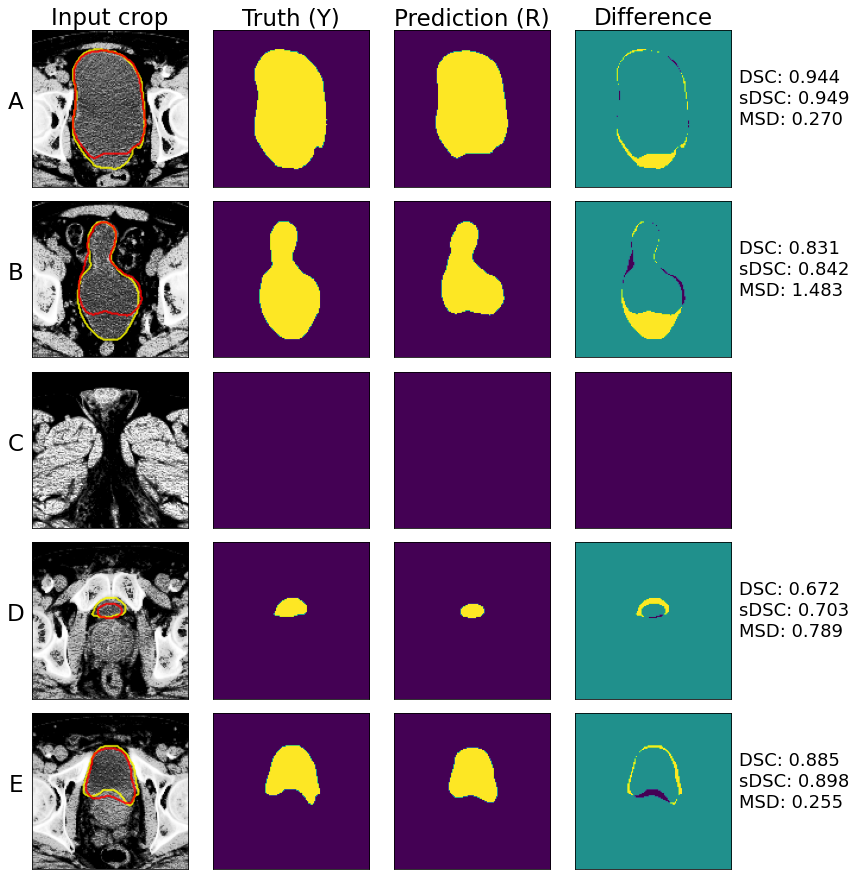
\includegraphics[width=1.0\textwidth]{figures/prostate_bladder}
		\caption{Representative output for bladder: Model 1 - trained via weighted soft dice (w. soft DSC) loss - 140 epochs. Truth contour (yellow), prediction contour (red). Mean surface distance (MSD) in mm. sDSC \cite{Nikolov_2018} calculated at an organ specific tolerance of $\tau$ = 1.46 mm, the 95th percentile mean surface distance between expert observers \cite{Roach_2019}.}
		\label{fig:prostate_bladder}
	\end{center}
\end{figure}

In Figure \ref{fig:prostate_bladder}, weighted soft DSC underestimated the posterior aspect of larger bladder examples - a recurrent limitation of the model. Figure \ref{fig:prostate_bladder} C) shows the model was correctly able to identify when contours were not present, indicating the strong negative predictive validity of the model - quantified by the high sensitivity score recorded on Table \ref{table:organ}.

\begin{figure}[H]
	\begin{center}
		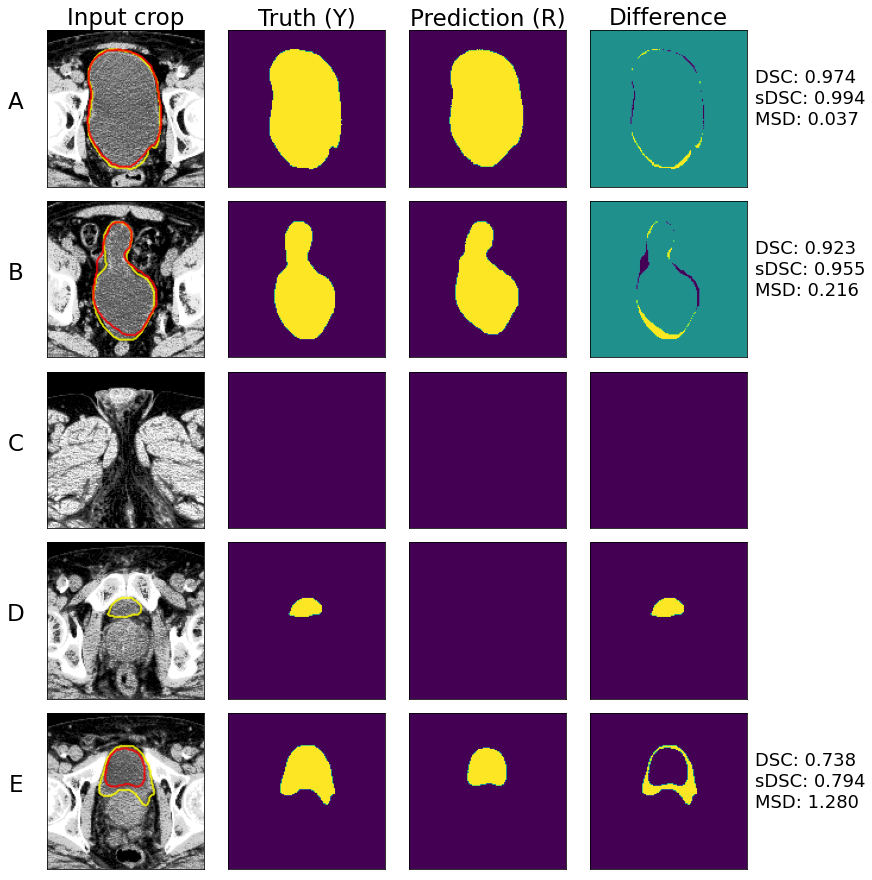
\includegraphics[width=1.0\textwidth]{figures/prostate_BCE_bladder}
		\caption{Representative model output for bladder: Trained via binary cross entropy loss - 78 epochs. Truth contour (yellow), prediction contour (red). Mean surface distance (MSD) in mm. sDSC \cite{Nikolov_2018} calculated at an organ specific tolerance of $\tau$ = 1.46 mm, the 95th percentile mean surface distance between expert observers \cite{Roach_2019}.}
		\label{fig:prostate_BCE_bladder}
	\end{center}
\end{figure}

Model 1 under weighted soft DSC was unable to identify rectum contours containing hollow regions (see Figure \ref{fig:prostate_rectum} D). We suspect further training on a distribution of similar cases may improve performance. All other cases in the test dataset were correctly identified. As seen in Figure \ref{fig:prostate_rectum} and Table \ref{table:organ}, DSC values for rectum contours were lower on average when compared to the bladder - consistent with expert IOV \cite{CITATION}\todo[color=red!40]{Cite} and other models in the literature \cite{CITATION}\todo[color=red!40]{Cite}. However, a higher surface dice similarity coefficient (sDSC) indicated that the degree of correction required for rectum contours was lower than corrections required for bladder contours.


\begin{figure}[H]
	\begin{center}
		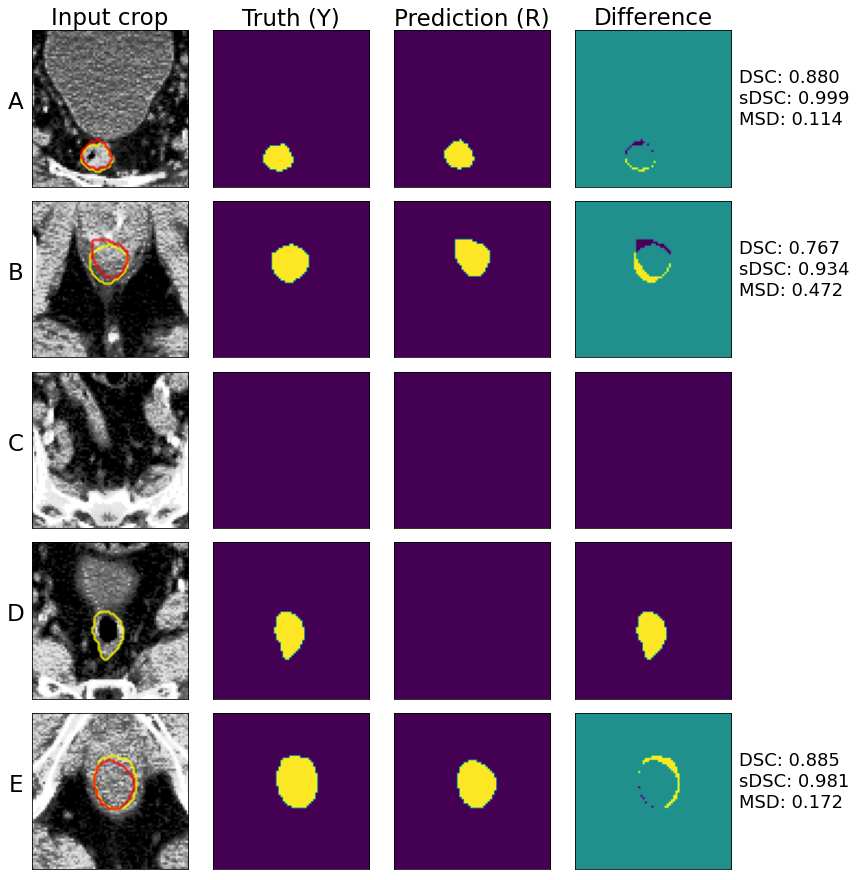
\includegraphics[width=1.0\textwidth]{figures/prostate_rectum}
		\caption{Representative output for rectum: Model 1 - trained via weighted soft dice (w. soft DSC) loss - 140 epochs. Truth contour (yellow), prediction contour (red). Mean surface distance (MSD) in mm. sDSC \cite{Nikolov_2018} calculated at an organ specific tolerance of $\tau$ = 6.99 mm, the 95th percentile mean surface distance between expert observers \cite{Roach_2019}.}
		\label{fig:prostate_rectum}
	\end{center}
\end{figure}

\section{Model 2: Canine imaging}

3 loss functions were attempted for vacuum bag segmentation in canine imaging, as seen in Table \ref{table:loss_vet}. Soft DSC outperformed both BCE and focal Tversky on DSC and precision values. Focal Tversky had the highest sensitivity (0.969) as expected \cite{Khan2019}, with BCE second (0.954). The final model was selected at 100 epochs under soft DSC loss. Representative model output is presented in Figure \ref{fig:vet_vacbag}. Soft DSC loss showed excellent agreement with ground truth vacuum bag contours - and was able to handle both negative (E) and small contour (B) examples in the test dataset (see Figure \ref{fig:vet_vacbag}).

\begin{table}[h]
\footnotesize
\caption{Loss evaluation on independent test dataset for canine imaging}
% title of Table
\centering
% used for centering table
\begin{tabular}{c c c c}
% centered columns (4 columns)
\hline\hline
%inserts double horizontal lines
Loss & DSC & Precision & Sensitivity \\ [0.5ex]
% inserts table
%heading
\hline
% inserts single horizontal line
BinaryCrossentropy & 0.901 & 0.935 & 0.954 \\
\textbf{soft DSC} & \textbf{0.952} & \textbf{0.953} & \textbf{0.953} \\
FocalTversky & 0.930 & 0.906 & 0.969 \\
% [1ex] adds vertical space
\hline\hline
%inserts single line
\end{tabular}
\label{table:loss_vet}
% is used to refer this table in the text
\end{table}


\begin{figure}[H]
	\begin{center}
		\hspace*{-1.2cm}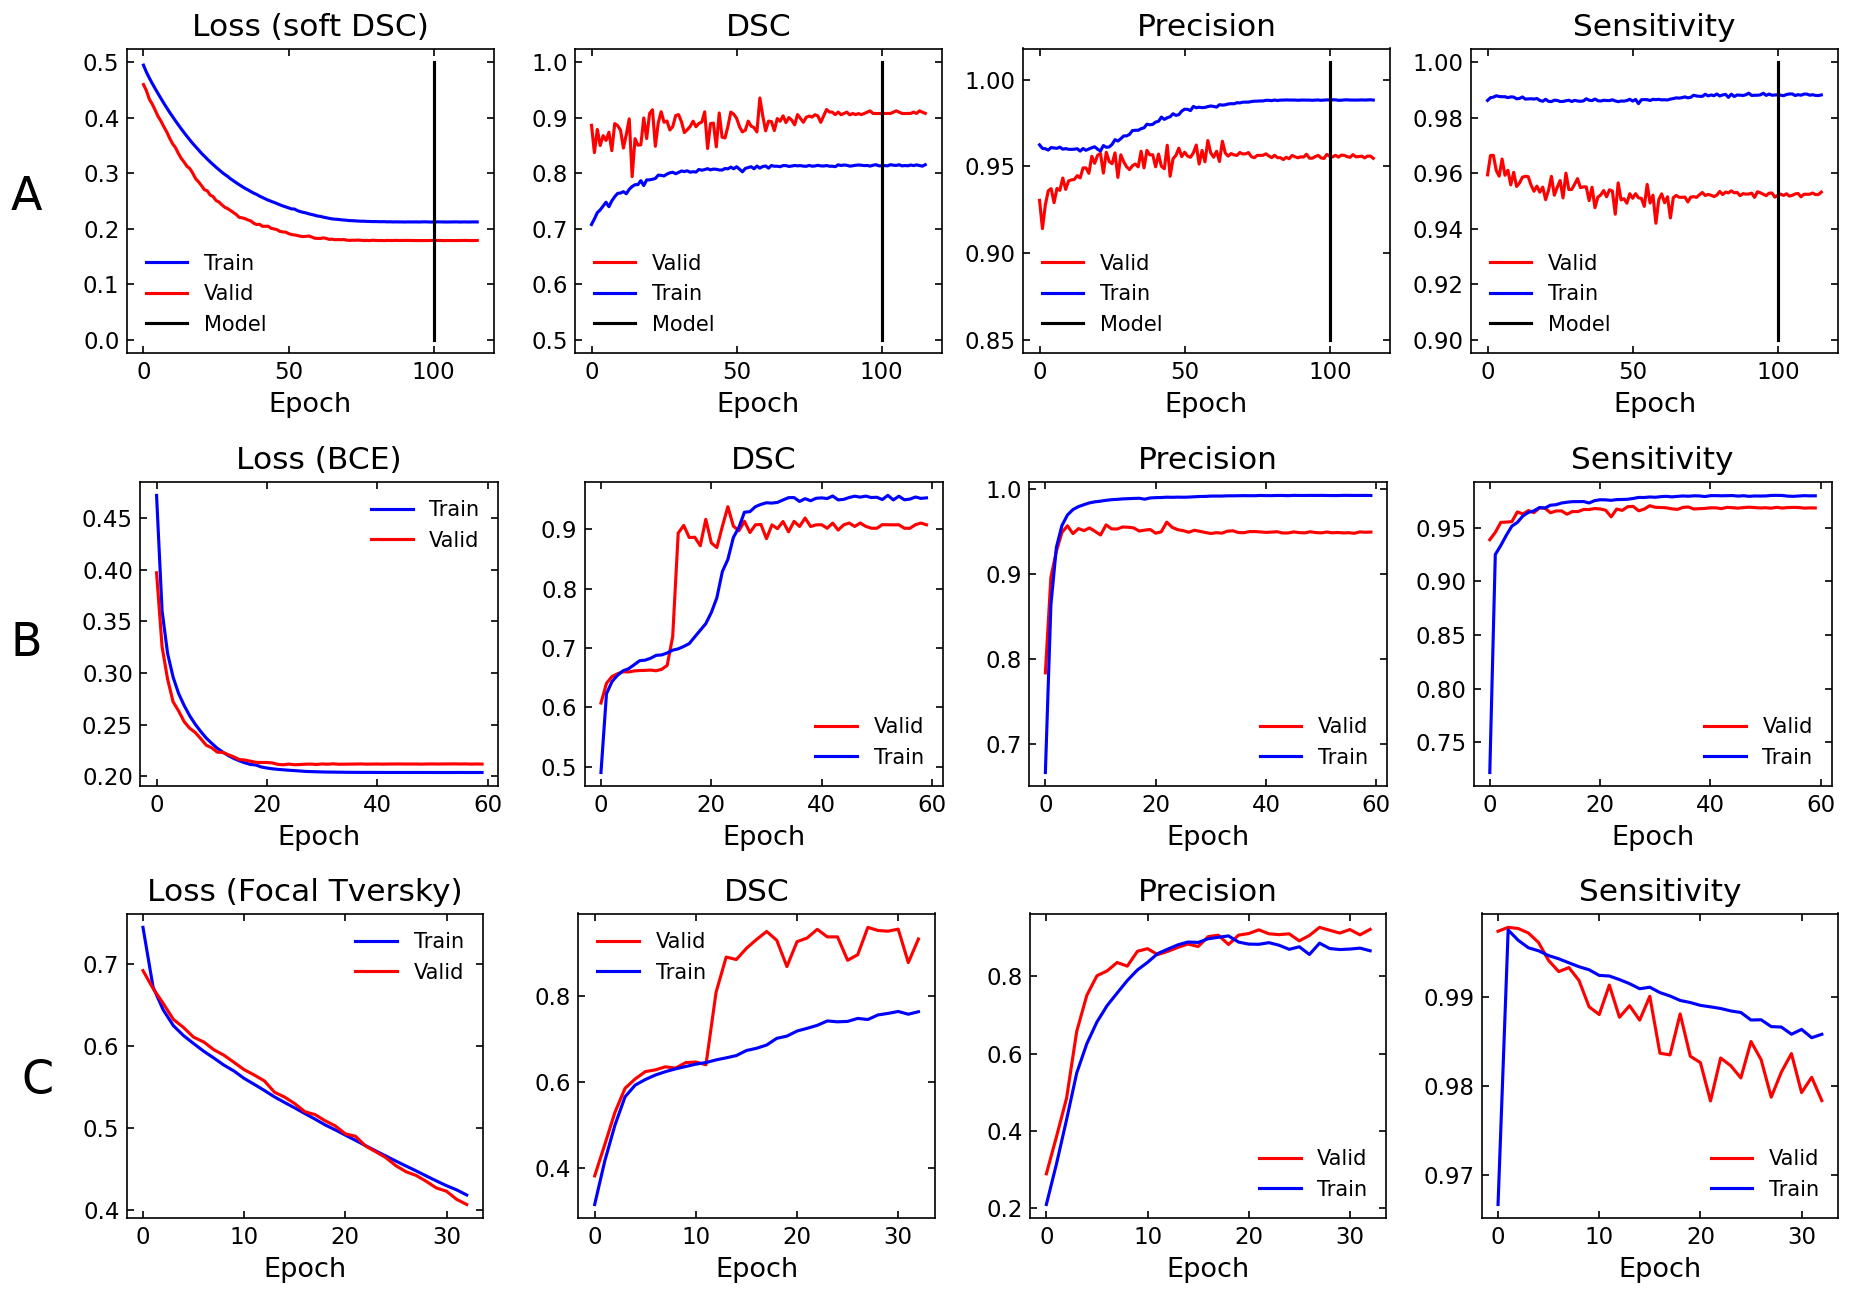
\includegraphics[width=1.15\textwidth]{figures/vacbag_metrics_combined}
		\caption{\textbf{A)} Model training metrics for canine imaging via soft dice similarity coefficient (soft DSC) loss. Final model selected at epoch 100 due to validation loss plateau. Training time 6 hours.\\
		\textbf{B)} Binary cross entropy (BCE) loss\\
		\textbf{C)} Focal Tversky loss}
		\label{fig:vet_metrics}
	\end{center}
\end{figure}

Typically, we expect training metric values to overstate a model's predictive capacity, as parameter values are updated to fit the training data distribution. However, in Figure \ref{fig:vet_metrics} we see that at many stages, validation loss was lower than training loss. The literature states two possible contributing factors: 1) Dropout layers regularise only on the training data, and hence the full architecture is only available for inference on the validation and testing sets \cite{srivastava2014}. Additionally, batch normalisation parameters are tuned to normalise activations on the test dataset - and are fixed during validation and testing \cite{CITATION}\todo[color=red!40]{Cite}. 2) Due to the small dataset used in this study, variation in the validation set may itself be small compared to the training data; hence, if the validation distribution is centred about the mean of the training data, the validation dataset would be relatively `easier' to infer \cite{CITATION}\todo[color=red!40]{Cite}. We note that although Tversky loss continued to decrease for both the training and validation sets over the epochs tested, a DSC validation plateau (see oscillation in Figure \ref{fig:vet_metrics} C)) triggered early stopping.

\begin{figure}[H]
	\begin{center}
		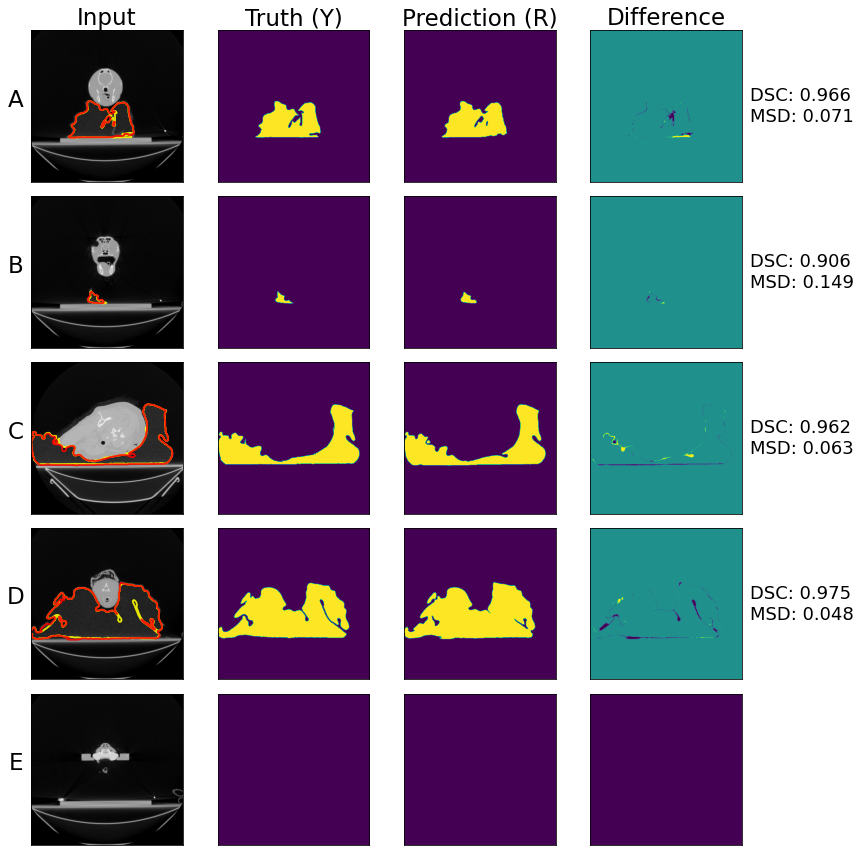
\includegraphics[width=1.0\textwidth]{figures/vet_vacbag}
		\caption{Representative output for vacuum bag: Model 2 - trained soft DSC loss. Truth contour (yellow), prediction contour (red). Mean surface distance (MSD) mm.}
		\label{fig:vet_vacbag}
	\end{center}
\end{figure}

\section{Clinical relevance}
The pelvic imaging model showed excellent agreement with observers for patient contours, with an average DSC value of 0.998, and a mean surface distance (MSD) of $<0.1$ mm, as seen in Table \ref{table:organ}. Bladder contours had an average DSC score of 0.864 with a standard deviation (STD) of 0.221. Additionally, average bladder MSD was measured to be 1.075 mm with an STD of 2.986 mm. Average volumetric rectum agreement was considerably lower, with an average DSC of 0.670 and STD 0.121, and a MSD of 1.120 mm with STD 2.143 mm. In comparison, organ specific tolerances used for these OARs (95th percentile MSD between experts - i.e. top 95\% expert variance) were determined to be 1.46 mm and 6.99 mm for the bladder and rectum, respectively \cite{Roach_2019, Nikolov_2018}. Large variances in bladder MSD corresponded to predictions that under-segmented the posterior aspect of the bladder (as seen in Figure \ref{fig:prostate_bladder} A-B) However, the vast majority of bladder surfaces were contoured correctly within expert IOV - with a mean sDSC 0.876(0.117). In comparison, an even larger proportion of rectum surface points did not need correction to be within expert IOV, with a mean sDSC of 0.922(0.138) recorded. More work is required to correlate sDSC values with time required for contour correction \cite{Nikolov_2018, Vaassen_2020}.

Literature reports that clinically acceptable agreement between expert observers is DSC $\geq$ 0.7 for the bladder and rectum \cite{Roach_2019}. However, experts have been reported to acheive similarities much higher than this,  DSC 0.93 $\pm$ 0.03, MSD 0.99(0.30) mm for the bladder and DSC 0.81 $\pm$ 0.07, MSD 2.862(2.066) mm for the rectum \cite{Roach_2019}. These finding indicate that although rectum contours produced by model 1 may be clinically acceptable, model performance falls short of expert IOV without contour correction. 

State-of-the-art U-net implementations have recently been able to achieve DSC values of 0.95 and 0.92 for the bladder and rectum, respectively \cite{Kazemifar_2018}. However, 85 CT patient scans were included in this dataset, compared to the 16 included in our study. We suspect that increasing the number of patients in our study would lead to higher generalisability in model performance (reported to scale logarithmically with dataset size \cite{Nemoto_2020}) as well as provide a broader validation and test distribution - improving the reliability and robustness of performance metrics \cite{Ronneberger_2015}. 

Model 2 produced vacuum bag contours with an average DSC of 0.952 and MSD of 0.175 mm with STD of 0.275 mm. The vacuum bag material has an electron density of approximately 0.1\% of water \cite{CITATION}\todo[color=red!40]{Cite}; hence, the 95th percentile vacuum bag MSD (0.726 mm) corresponds to a negligible shift is dose distribution under contours produced by this model - and a potential time saving of 30 minutes per patient. Dose shift has yet to be assessed  in clinic - however, we suggest that comparing dose volume histograms between model and expert contours under an identical treatment plan could provide a quantitative measure of clinical acceptability. If acceptance testing validates vacuum bag segmentation, model 2 has the potential to save approximately 30 minutes in treatment planning time per patients \cite{CITATION}\todo[color=red!40]{Cite}.

\begin{table}[H]
\footnotesize
\caption{Organ specific evaluation for proposed models on independent test dataset}
\centering
\begin{tabular}{c c c c c c}
\hline\hline
Organ: Mean(Std) & sDSC ($\tau$) & DSC  & MSD (mm) & Sensitivity & Specificity \\ [0.5ex]
\hline
\textbf{Pelvic imaging} &              &              &              &       &       \\
Patient   &             & 0.998(0.001) & 0.002(0.005) & 0.997 & 0.999 \\
Bladder ($\tau$ 1.46 mm) [2] & 0.876(0.177) & 0.864(0.221) & 1.075(2.986) & 0.786 & 0.999 \\
Rectum ($\tau$ 6.99 mm) [2]  & 0.922(0.138) & 0.670(0.121) & 1.120(2.143) & 0.619 & 0.999 \\
Average                  &             & 0.994(0.153) & 0.409(1.604) & 0.991 & 0.999 \\ \\
\textbf{Canine imaging} &              &              &              &       &       \\
Vacbag    &              & 0.952(0.001) & 0.176(0.275) & 0.953 & 0.995\\
\hline\hline
\end{tabular}
\label{table:organ}
\end{table}


\todo[inline, color=blue!40]{Addition? Further discuss dose implications. Yaser wanted to see this but i feel like this is tangential to the main points of this report. To assess properly would be a project in itself - its also not discussed in ML lit.}


\section{Limitations and future work}

A common challenge in deep-learning applications to medical imaging is small data set sizes \cite{Ronneberger_2015}. Limited data reduces model generalisability \cite{Shen2017}. With state-of-the-art implementations using up to 1000 patients per study \cite{Nikolov_2018}, we expect our results for bladder and rectum segmentation could improve significantly with the broader distribution provided by a larger dataset.

Additionally, organ-specific tolerances used in this study were acquired by Roach et al. from 15 expert observers (9 of which were radiation oncologists) averaged over a cohort of 5 patients \cite{Roach_2019}. Reliability in these values could be improved by surveying a broader range of experts and patients.

To best of our knowledge, only 1 attempt to correlate sDSC with the time required for contour correction currently exists in the literature. Therefore, more work is required to assess the utility of sDSC in a clinical workflow. Alternative surface-based metrics have also been presented; for example, the estimated added path length in Vaassen et al. (seen in Figure \ref{fig:vaassen}). However, no study currently exists comparing sDSC and estimated added path length under IOV tolerances. Additionally, there is an opportunity to investigate the barriers and limitations in designing a soft surrogate sDSC metric that can be optimised directly during training.

Furthermore, our ultimate responsibility lies in improving patient outcomes. Hence, there is an opportunity to correlate DSC and sDSC performance with changes to dose distribution when compared with plans developed under expert contouring. A potential advantage of sDSC compared to DSC is the stronger correlation with the time required for contour correction - however, correlation with dose shift may also be an important clinical indicator.

Current studies are researching potential improvements in medical imaging segmentation under 3D U-net models. Although this study focused on a 2D implementation due to the clinical barriers inherent in 3D models, more work is still required to quantify the potential for performance improvement. 

\chapter{Conclusion}
\label{ch:conclusion}

This study attempted 2D U-Net architecture with a small dataset and image augmentation. Performance was assessed under a variety of standard loss functions used in semantic segmentation tasks. Two models were developed: Model 1 aimed to contour the patient, bladder, and rectum structures in pelvic CT images, to provide a QA tool for background contour monitoring RT. Additionally, we provided surface dice similarity coefficients for the bladder and rectum contours, with organ-specific tolerances at the 95th percentile mean surface distance between expert observers. Model 2 aimed to automate the contouring of vacuum bags in canine imaging for RT, a time-consuming structure that is delineated manually at SASH veterinary clinic.

Weighted soft DSC loss was selected for the pelvic imaging model as it was the only loss that overcame the class imbalance in our data, to optimise for all OARs in the model output. Patient contours were clinically acceptable DSC of 0.998. However, it is suspected that more data will be required to improve bladder and rectum segmentation before clinical use as a QA tool, with DSCs of 0.860 and 0.670, respectively.

 However, the surface dice similarity coefficient indicated that the majority of bladder and rectum surfaces were within expert IOV, with sDSCs of 0.876 and 0.922, respectively

Soft DSC loss was selected for the canine imaging model, which produced (likely)

\todo[inline]{Instead of saying (likely) here, a statement that leans on your PDD calculations done above would end up saying something like, the deviations in dose induced by using the auto-contoured vac bag model are never more than 0.1\% for any given ray line through the vac bag. Given many gantry angles are used, and there is not a significant systematic error within the vac-bag contouring, and under no circumstance was a vac-bag not contoured when in fact it was there, it is able to be rolled out for clinical use at SASH under the condition that a human operator still investigates the contours. It is expected that little to no correction should be needed during regular use}

acceptable vacuum bag contouring with a DSC of 0.952. As this model has the potential to save 30 minutes of planning time per patient, further work will involve clinical acceptance testing and implementation.




% % ================= BACK MATTER =========================
\backmatter
% BIBLIOGRAPHY 
\small{\printbibliography[title=References]}
  %\bibliography{/home/matthew/masters_articles/references.bib}
  %\bibliographystyle{ieeetr}
% APPENDIX
% \appendix
%\chapter{Appendix}
\label{ch:appendix}



\end{document}